\documentclass[12pt,a4paper,twoside]{article}
\usepackage{fancyhdr}
\usepackage{lastpage}
\usepackage[top=2.5cm, bottom=2.5cm, left=2.5cm, right=2.5cm]{geometry} % Marges strictes ENSIMAG (2.5cm max)
\usepackage{amsmath}
\usepackage{amssymb} 
\usepackage{graphicx}
\usepackage{color}
\usepackage{fancybox}
\usepackage{moreverb}
\usepackage{listings}
\usepackage{subcaption}
\usepackage{siunitx}
\usepackage[utf8]{inputenc}
\usepackage[T1]{fontenc}
\usepackage[french]{babel}
\usepackage{hyperref}
\usepackage{pgfgantt}
\usepackage{booktabs}
\usepackage{float}
\usepackage{booktabs}
\usepackage{changepage}
\usepackage{multirow}
\usepackage[table]{xcolor}
\usepackage[backend=biber, style=numeric, sorting=none]{biblatex}
\addbibresource{biblio.bib}
\definecolor{barblue}{RGB}{79, 129, 189}
\definecolor{linkred}{RGB}{192, 0, 0}
\definecolor{groupgray}{RGB}{90, 90, 90}
\definecolor{gridgray}{RGB}{230, 230, 230}

% --- Configuration de Fancyhdr (En-têtes et pieds de page) ---
\pagestyle{fancy}
\fancyhf{} 
\fancyhead[LE,RO]{\footnotesize\itshape\leftmark} 
\fancyfoot[C]{\thepage\ / \pageref{LastPage}} 
\renewcommand{\headrulewidth}{0.4pt} 
\renewcommand{\footrulewidth}{0pt}  

\begin{document}
\lstset{ numbers=left, tabsize=3, frame=single, numberstyle=\ttfamily, basicstyle=\footnotesize} 

% --- PAGE DE GARDE ---
\thispagestyle{empty}
\begin{center}
\makebox[\textwidth][l]{
\raisebox{-40pt}[0pt][0pt]{

\includegraphics[scale=0.18]{logo_inrae.pdf}
}
}
\makebox[\textwidth][r]{
\raisebox{0pt}[0pt][0pt]{

\includegraphics[scale=0.2]{logo_ensimag.pdf}
}
}
\vspace{1cm}
Grenoble INP  -- ENSIMAG\\
École Nationale Supérieure d'Informatique et de Mathématiques Appliquées\\
\vspace{2cm}
{\LARGE Pré-rapport de projet de fin d'études}\\
\vspace{0.8cm}
Effectué chez\\
\textbf{INRAE}\\
Institut National de Recherche pour l'Agriculture, l'Alimentation et l'Environnement\\
\vspace{1cm}
\shadowbox{
\begin{minipage}{0.95\textwidth}
\begin{center}
\vspace{0.3cm}
{\Large\bfseries Exploitation de signaux RMN par apprentissage profond pour la caractérisation d'états physiologiques des plantes}
\vspace{0.3cm}
\end{center}
\end{minipage}
}\\
\vspace{1.5cm}
\textbf{Gabriel Poirier}\\
3e année -- Option ISI\\
Filière Ingénierie des Systèmes d'Information\\
\vspace{2mm}
Avril 2026 -- Septembre 2026\\
\vspace{1.5cm}

% --- FICHE DE COORDONNÉES EXIGÉE ---
\begin{tabular}{p{5.5cm}p{5.5cm}p{5.5cm}}
\textbf{Étudiant} & \textbf{Structure d'accueil} & \textbf{Tuteur Enseignant} \\
Gabriel Poirier & INRAE -- AgroResonance & Patrick Reignier \\
ENSIMAG - Option ISI & Route de Theix & ENSIMAG \\
\footnotesize \href{mailto:gabriel.poirier@grenoble-inp.org}{gabriel.poirier@grenoble-inp.org} & \footnotesize 63122 Saint-Genès-Champanelle & \footnotesize \href{mailto:patrick.reignier@grenoble-inp.fr}{patrick.reignier@grenoble-inp.fr} \\
& \footnotesize Tuteur : Jean-Marie Bonny & \\
& \footnotesize \href{mailto:jean-marie.bonny@inrae.fr}{jean-marie.bonny@inrae.fr} & \\
\end{tabular}
\end{center}

\clearpage

% --- RÉSUMÉ ET MOTS CLÉS ---
\thispagestyle{plain}
\section*{Résumé}

Ce projet de fin d'études porte sur l'analyse automatique de signaux de Résonance
Magnétique Nucléaire (RMN) bas champ pour la caractérisation de l'état
physiologique des plantes. L'objectif est de développer un pipeline de traitement
et d'apprentissage profond permettant d'exploiter des acquisitions RMN
individuelles, malgré leur faible rapport signal sur bruit, afin de détecter des
variations physiologiques telles que les cycles circadiens et le stress hydrique.

Une chaîne complète de traitement a été développée, comprenant l'extraction de
régions d'intérêt, la détection des acquisitions aberrantes et différentes
architectures de réseaux convolutifs. Pour les signaux représentés sous forme
unidimensionnelle, une architecture hybride combinant un CNN 1D et des
métadonnées environnementales a été étudiée, ainsi qu'une architecture
multi-têtes permettant de prendre en compte la variabilité inter-espèces.

Le travail étudie également l'exploitation de données RMN simulées comme source
de pré-entraînement. Plusieurs stratégies de transfert vers les données
expérimentales sont comparées, du transfert sans adaptation (\textit{zero-shot})
au \textit{fine-tuning}. Ces expériences montrent que les données simulées
contiennent une information discriminante exploitable, mais ne reproduisent pas
à elles seules toute la complexité des acquisitions expérimentales.

Enfin, une architecture convolutive 2D est développée pour exploiter directement
la dimension spatiale de signaux RMN acquis sur des troncs d'arbres soumis à un
stress hydrique. L'utilisation d'une optimisation bayésienne permet d'adapter
automatiquement les hyperparamètres du modèle, tandis que l'utilisation de
Grad-CAM++ fournit des éléments d'interprétation des régions du signal utilisées
par le réseau.

L'ensemble de ces travaux montre l'intérêt d'une approche combinant traitement
du signal, apprentissage profond et explicabilité pour l'analyse non destructive
de l'état physiologique des plantes.

\vspace{1cm}
\noindent \textbf{Mots-clés :} Résonance Magnétique Nucléaire (RMN), Spécificités végétales, Apprentissage Profond, Réseaux de neurones convolutifs 1D, Détection d'anomalies, PyTorch.

\clearpage

% --- GLOSSAIRE ---
\thispagestyle{plain}
\section*{Glossaire}
\begin{description}
    \item[1D-CNN] \textit{One-Dimensional Convolutional Neural Network}. Réseau de neurones convolutif adapté au traitement de structures séquentielles ou de signaux temporels unidimensionnels.
    \item[CPMG] Séquence d'impulsions de \textit{Carr-Purcell-Meiboom-Gill}. Protocole physique d'acquisition RMN mesurant la décroissance de la relaxation transversale $T_2$.
    \item[INRAE] Institut National de Recherche pour l'Agriculture, l'Alimentation et l'Environnement.
    \item[K-Fold] Méthode de validation croisée (\textit{Cross-Validation}) consistant à diviser le jeu de données en $K$ morceaux (\textit{folds}) de tailles égales, afin de répéter l'entraînement $K$ fois en changeant le lot de validation à chaque itération pour fiabiliser l'évaluation des performances.
    \item[Fold] (ou Pli). Sous-ensemble de données disjoint issu du partitionnement d'un jeu de données initial, utilisé alternativement comme base d'entraînement ou de validation.
    \item[KNN] \textit{$K$-Nearest Neighbors} (K-plus proches voisins). Algorithme d'apprentissage utilisé ici pour la détection locale d'anomalies.
    \item[MLP] \textit{Multi-Layer Perceptron} (Perceptron Multicouche). Architecture de réseau de neurones standard entièrement connectée.
    \item[NMR MOUSE] \textit{Mobile Universal Surface Explorer}. Capteur RMN unilatéral bas champ transportable utilisé pour les mesures de surface non destructives.
    \item[ROI] \textit{Region Of Interest} (Région d'Intérêt). Portion utile d'un signal ou d'une matrice isolée pour l'analyse.
    \item[RMN] Résonance Magnétique Nucléaire. Technique physique exploitant les propriétés magnétiques de certains noyaux atomiques.
    \item[$SNR$] \textit{Signal-to-Noise Ratio} (Rapport Signal sur Bruit).
\end{description}

\clearpage

% --- TABLE DES MATIÈRES ---
\thispagestyle{plain}
\tableofcontents
\clearpage

% --- CORPS DU RAPPORT ---
\setcounter{page}{1} 

\section{Introduction et Contexte du Projet}
\label{sec:introduction}

\subsection{Contexte institutionnel et positionnement de la mission}
\label{subsec:contexte_institutionnel}

Ce Projet de Fin d'Études (PFE) s'inscrit dans le cadre de la dernière année de formation d'ingénieur à l'ENSIMAG, au sein de la filière Ingénierie des Systèmes d'Information (ISI). Le projet est réalisé au sein de l'INRAE (Institut National de Recherche pour l'Agriculture, l'Alimentation et l'Environnement), dans le centre Clermont-Auvergne-Rhône-Alpes. 

L'INRAE se place au cœur des enjeux contemporains liés à la transition agroécologique, à l'adaptation aux changements climatiques et à la sécurité alimentaire. Ce stage se situe à l'interface exacte des compétences en science des données de la filière ISI et des besoins de la recherche publique : mettre les outils avancés du traitement de signal et du \textit{Deep Learning} au service de la compréhension et de la modélisation du vivant.

\subsection{Enjeux agronomiques et problématique d'analyse}
\label{subsec:enjeux_agronomiques}
Face au changement climatique, la compréhension fine des mécanismes d'adaptation des plantes à leur environnement est devenue un levier crucial pour l'agriculture de précision. Ce travail s'articule autour de deux aspects physiologiques majeurs : la caractérisation du rythme circadien (alternance Jour/Nuit), qui régule l'activité métabolique fondamentale, et la détection précoce du stress hydrique, qui impacte directement la cinétique de croissance des cultures.

Pour obtenir des informations métaboliques in vivo sans perturber le fonctionnement de la plante, les méthodes destructives traditionnelles sont écartées au profit de la Résonance Magnétique Nucléaire (RMN) portable. Cependant, les signaux spatio-temporels bruts issus de ces mesures sur le vivant présentent un rapport signal sur bruit ($SNR$) extrêmement faible et une forte variabilité, rendant l'interprétation physique directe difficile. L'objectif central de ce projet est donc de concevoir un pipeline d'apprentissage profond permettant de classer les signaux RMN associés à des états métaboliques connus et d'identifier les composantes du signal responsables de la discrimination entre ces états.

\subsection{Phénomène de RMN et spécificités du capteur}
\label{subsec:rmn}
\subsubsection{Principe de la Résonance Magnétique Nucléaire}
La RMN repose sur l'interaction entre le moment magnétique (spin) de certains noyaux atomiques et des champs magnétiques externes. Placés dans un tel champ, les noyaux s'ordonnent partiellement, faisant apparaître une aimantation macroscopique au sein de l'échantillon. Une brève impulsion radiofréquence (RF) appliquée à la fréquence de résonance du noyau vient perturber cet équilibre. Lors de la phase de relaxation qui suit l'arrêt de l'impulsion, les spins reviennent à leur état d'équilibre en émettant un signal RF détectable. L'analyse de cette relaxation — notamment le temps de relaxation transversal $T_2$ — fournit des informations sur la dynamique de l'eau \cite{Levitt2013}.


\subsubsection{Le capteur NMR-MOUSE}

Le NMR‑MOUSE (\textit{Mobile Universal Surface Explorer}) \cite{Blumich1998} est un dispositif de RMN unilatéral et portable, adapté aux mesures \textit{in situ}. Contrairement aux imageurs médicaux ou de laboratoire qui confinent l'échantillon dans des champs intenses (\num{1.5} à \num{7}~T), ce capteur utilise un aimant permanent ouvert générant un champ faible d'environ \num{0.3}~T.
Cette configuration présente deux spécificités majeures :
\begin{itemize}
\item \textbf{Noyau cible :} En régime de bas champ, la détection est limitée aux noyaux d'hydrogène ($^1\text{H}$), qui possèdent la sensibilité intrinsèque la plus élevée en RMN. Ce noyau étant le constituant majeur de l'eau et donc des tissus végétaux, le NMR-MOUSE est particulièrement adapté à l'étude de la dynamique hydrique des plantes.
\item \textbf{Résolution spatiale :} L'ensemble aimant/antenne RF (cf. Figure~\ref{fig:MOUSE}) peut être déplacé à l'aide d'un ascenceur de précision. Ainsi, la zone sensible qui est une coupe fine peut varier au sein de l'échantillon. Le dispositif permet ainsi d'effectuer des mesures par tranches de profondeur successives, parallèles à la surface de l'aimant, avec une précision allant jusqu'à \num{50}~\textmu m. Il est ainsi possible d'acquérir le signal à différentes profondeurs.

\begin{figure}[htbp]
\centering
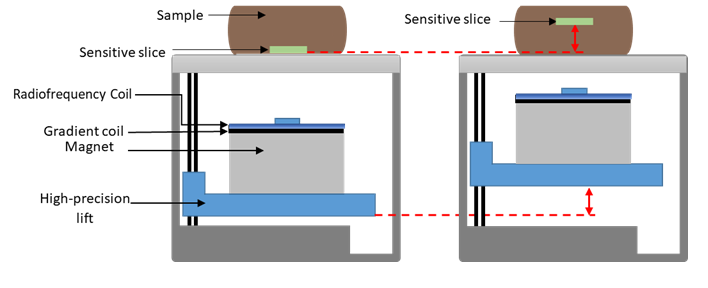
\includegraphics[scale=0.8]{MOUSE}
\caption{Schéma présentant le fonctionnement du NMR-MOUSE}
\label{fig:MOUSE}
\end{figure}

\end{itemize}

\subsection{Jeux de données exploités}
\label{subsec:donnees_intro}

Les travaux présentés dans ce rapport s'appuient sur deux jeux de données expérimentaux issus de travaux de recherche portant sur l'utilisation de la RMN pour caractériser la dynamique de l'eau dans les plantes. Le premier provient des travaux de thèse de M. Nuixe et est décrit notamment dans l'étude de Nuixe et al.~\cite{nuixe2024use}. Le second a été obtenu dans le cadre des travaux de thèse de S. Blystone~\cite{Shannan}.

\subsubsection{Jeu de données « Racines »}

Le premier jeu de données comprend \num{10} espèces d'herbacées : \textit{Dactylis glomerata} (espèce 1), \textit{Trifolium pratense} (espèce 2), \textit{Festuca arundinacea} (espèce 3), \textit{Lupinus angustifolius} (espèce 4), \textit{Medicago sativa} (espèce 5), \textit{Onobrychis viciifolia} (espèce 6), \textit{Plantago lanceolata} (espèce 7), \textit{Rumex acetosa} (espèce 8), \textit{Taraxacum officinale} (espèce 9) et \textit{Trifolium repens} (espèce 10).

Ces espèces ont été cultivées dans des \textit{rhizotrons}, des dispositifs vitrés permettant notamment l'observation et le suivi du système racinaire. Les mesures ont été acquises de manière non destructive à l'aide du capteur NMR-MOUSE. Celui-ci permet d'obtenir des courbes de décroissance de la relaxation transversale $T_2$ à l'aide d'une séquence CPMG comportant \num{256} échos~\cite{Meiboom1958}. Les mesures sont réalisées à différentes profondeurs, comprises entre \num{0}~mm, correspondant à la vitre, et \num{14.7}~mm dans le substrat, conduisant à des signaux de dimension $256 \times 148$. Chaque espèce a été mesurée entre 100 et 200 fois, avec un intervalle d'environ \num{40}~min entre deux acquisitions.

Le jeu de données présente ainsi trois dimensions d'évolution. La première est une dimension spatiale, correspondant à la profondeur de mesure au sein du rhizotron. La deuxième est une dimension temporelle à l'échelle de la milliseconde, correspondant au temps d'écho selon lequel évolue chaque signal de relaxation RMN. Enfin, une troisième dimension temporelle, à une échelle macroscopique de l'ordre de l'heure, permet de suivre l'évolution des signaux au cours du temps et notamment de mettre en évidence des variations liées au cycle circadien.

La composante spatiale permet notamment de localiser la présence d'eau dans le système expérimental. Le signal RMN présente ainsi une forte concentration à une profondeur correspondant à la position de la racine, qui constitue la principale composante du système expérimental contenant une quantité importante d'eau. La Figure~\ref{fig:signal_complet} présente différentes représentations de ces trois dimensions (notamment l'organisation 3D sur la Figure~\ref{fig:volume3D}, le profil spatial sur la Figure~\ref{fig:profil_profondeur} et le profil temporel sur la Figure~\ref{fig:profil_temps}). Le signal de relaxation observé dans la racine présente une décroissance généralement multiexponentielle. La figure présente ici un signal moyen calculé à partir des mesures réalisées sur \textit{Dactylis glomerata}.

\begin{figure}[htbp]
\centering

\begin{subfigure}{0.95\textwidth}
    \centering
    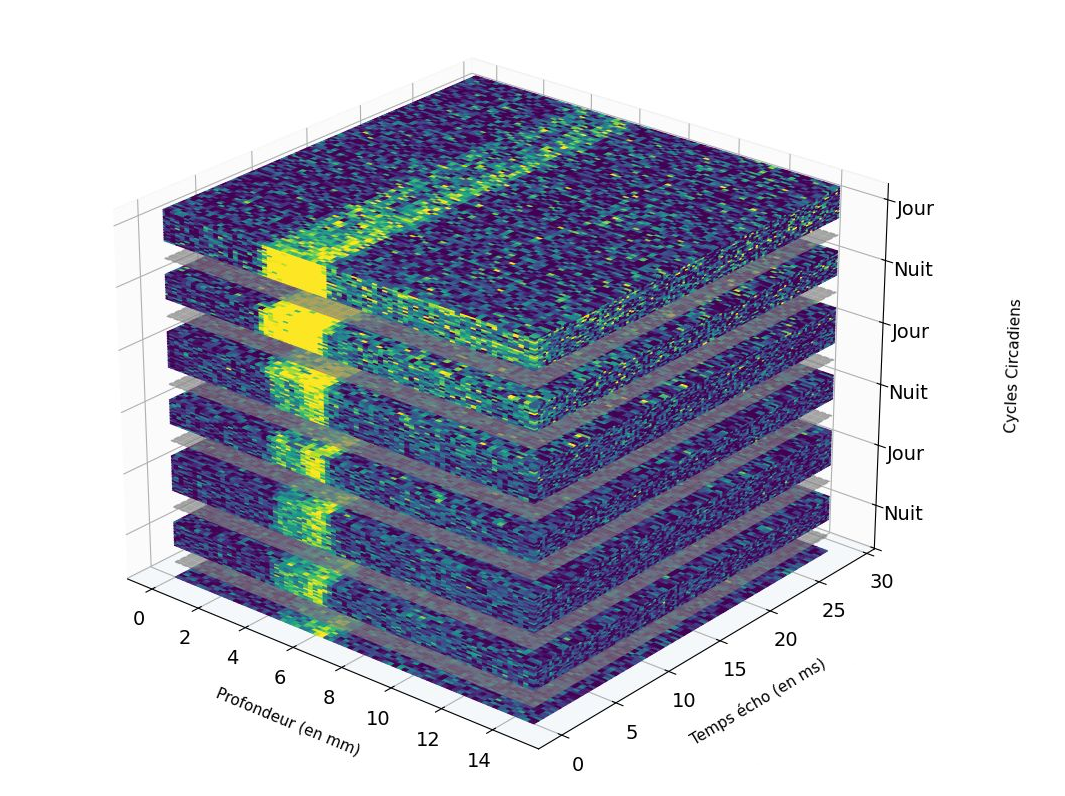
\includegraphics[width=\textwidth]{volume3D}
    \caption{Volume 3D du signal en fonction de la profondeur, du temps d'écho et du numéro de mesure.}
    \label{fig:volume3D}
\end{subfigure}

\vspace{0.5cm}

\begin{subfigure}{0.48\textwidth}
    \centering
    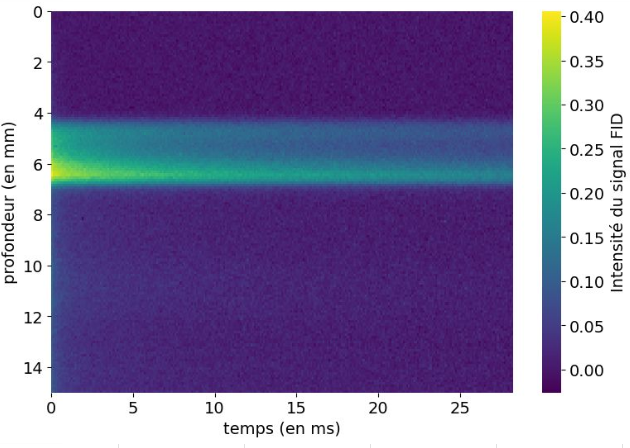
\includegraphics[width=\textwidth]{profil_profondeur}
    \caption{Signal moyen en fonction du temps d'écho et de la profondeur.}
    \label{fig:profil_profondeur}
\end{subfigure}
\hfill
\begin{subfigure}{0.48\textwidth}
    \centering
    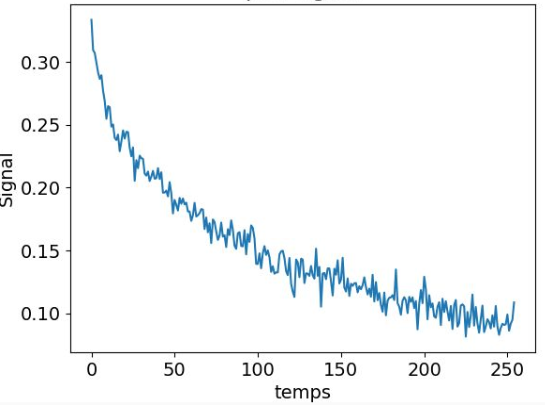
\includegraphics[width=\textwidth]{profil_temps}
    \caption{Signal moyen en fonction du temps d'écho, dans la racine.}
    \label{fig:profil_temps}
\end{subfigure}

\caption{Différentes représentations du signal mesuré sur \textit{Dactylis glomerata}.}
\label{fig:signal_complet}

\end{figure}

Sur la base des performances obtenues lors des premières expérimentations, un sous-ensemble de référence a été constitué à partir des espèces 1, 6, 9 et 10. Dans la suite de ce rapport, ce jeu de données sera désigné sous le nom de jeu de données « Racines ».

\subsubsection{Jeu de données « Tronc »}

Le second jeu de données, issu des travaux de S. Blystone~\cite{Shannan}, porte sur l'étude de la dynamique hydrique des parties aériennes des plantes à l'aide d'un capteur RMN portable et unilatéral. Contrairement au jeu de données « Racines », les mesures sont ici réalisées sur les troncs d'arbres. Dans le cadre de notre étude, le jeu de données exploité comprend cinq arbres appartenant à une même espèce, mesurés quotidiennement au cours de l'expérience. Parmi ces cinq individus, trois sont soumis à un stress hydrique tandis que deux sont maintenus dans des conditions témoins.

Pour chaque arbre, les acquisitions RMN permettent d'obtenir un signal dépendant à la fois du temps d'écho et de la profondeur de mesure. Chaque acquisition est ainsi représentée sous la forme d'une matrice de dimension $512 \times 128$, correspondant respectivement aux \num{512} temps d'écho et aux \num{128} positions spatiales. La profondeur explorée par le capteur atteint environ \num{15}~cm, permettant de caractériser la distribution du signal RMN à travers une partie importante du tronc.

Les mesures étant réalisées quotidiennement sur les mêmes individus, le jeu de données possède également une dimension temporelle macroscopique. Chaque arbre est ainsi observé de manière longitudinale, ce qui permet de suivre l'évolution de son état hydrique au cours de l'expérience et notamment d'observer les différences entre les arbres soumis au stress hydrique et les arbres témoins.

Le jeu de données présente donc trois dimensions d'évolution : une dimension spatiale correspondant à la profondeur dans le tronc, une dimension temporelle à l'échelle de la milliseconde correspondant au temps d'écho de la séquence de relaxation RMN, et une dimension temporelle macroscopique correspondant aux différents jours de mesure. Cette organisation permet de représenter les acquisitions sous la forme d'un volume de données, dans lequel chaque coupe selon les deux premières dimensions correspond au profil RMN d'un arbre à une date donnée.

Cette structure multidimensionnelle constitue un intérêt majeur pour notre étude. Contrairement au jeu de données « Racines », pour lequel l'information spatiale est principalement utilisée pour localiser la racine, les mesures réalisées sur les troncs permettent d'exploiter directement la distribution spatiale du signal au sein de l'échantillon. L'objectif est donc d'étudier dans quelle mesure cette information spatiale peut être intégrée aux modèles d'apprentissage automatique, en complément de la dynamique de relaxation du signal, afin de mieux caractériser l'état hydrique des arbres.

Dans la suite de ce rapport, ce jeu de données sera désigné sous le nom de jeu de données « Tronc ».

\subsection{Objectifs scientifiques}
\label{subsec:objectifs_projet}

L'objectif général de ce projet est d'étudier dans quelle mesure les signaux
RMN bas champ peuvent être exploités automatiquement pour caractériser l'état
physiologique des plantes à l'aide de méthodes d'apprentissage profond.

Cette problématique se décline en plusieurs objectifs complémentaires :

\begin{enumerate}
    \item \textbf{Exploiter les acquisitions individuelles :}
    développer une chaîne de traitement permettant d'extraire et de nettoyer
    les signaux RMN individuels malgré leur faible rapport signal sur bruit.

    \item \textbf{Développer des modèles adaptés aux signaux RMN :}
    concevoir des architectures convolutives capables d'extraire
    automatiquement des caractéristiques discriminantes à partir des courbes
    de relaxation, tout en prenant en compte les métadonnées environnementales
    et la variabilité inter-espèces.

    \item \textbf{Évaluer l'apport des données simulées :}
    déterminer si des signaux RMN simulés peuvent être utilisés pour pré-entraîner
    les modèles et dans quelle mesure les représentations ainsi apprises sont
    transférables aux données expérimentales.

    \item \textbf{Exploiter la dimension spatiale :}
    étudier un modèle convolutif 2D permettant de conserver simultanément les
    dimensions temporelle et spatiale lorsque cette dernière apporte une
    information physiologique pertinente.

    \item \textbf{Interpréter les décisions du modèle :}
    utiliser des méthodes d'explicabilité telles que Grad-CAM et Grad-CAM++
    afin d'identifier les régions des signaux utilisées par les réseaux et
    d'évaluer leur cohérence avec les phénomènes physiques étudiés.

    \item \textbf{Automatiser la recherche de modèles performants :}
    mettre en place une optimisation bayésienne des hyperparamètres afin
    d'identifier efficacement des configurations adaptées aux différents types
    de signaux étudiés.
\end{enumerate}

\subsection{Contribution personnelle}
\label{subsec:contribution_perso}

Ma contribution au projet couvre l'ensemble de la chaîne allant du traitement des
acquisitions RMN jusqu'à l'analyse et l'interprétation des modèles
d'apprentissage profond. Les différentes contributions peuvent être distinguées
selon les jeux de données auxquels elles s'appliquent.

\paragraph{Contributions communes aux deux jeux de données.}
Les travaux suivants ont été réalisés sur l'ensemble des données exploitées,
qu'elles proviennent du jeu « Racines » ou du jeu « Tronc » :

\begin{enumerate}
\item le développement de méthodes de définition et d'extraction des régions
d'intérêt dans les acquisitions RMN ;

\item l'étude et l'intégration de méthodes de détection des acquisitions
aberrantes afin d'améliorer la robustesse des jeux de données ;

\item l'implémentation d'une optimisation bayésienne des hyperparamètres
afin d'automatiser la recherche de configurations performantes ;

\item l'implémentation et l'adaptation de méthodes d'explicabilité, notamment
Grad-CAM et Grad-CAM++, afin d'analyser les régions des signaux utilisées
par les modèles.

\end{enumerate}

\paragraph{Contributions spécifiques au jeu « Racines ».}
Les travaux suivants ont été développés spécifiquement pour l'exploitation du
jeu de données « Racines » :

\begin{enumerate}
\item le développement sous PyTorch d'architectures convolutives 1D intégrant
notamment les caractéristiques des signaux, les métadonnées expérimentales
et une stratégie de classification multi-têtes ;

\item l'étude du transfert de connaissances entre données RMN simulées et
données expérimentales selon plusieurs stratégies de pré-entraînement et
de fine-tuning.

\end{enumerate}

\paragraph{Contribution spécifique au jeu « Tronc ».}
Enfin, l'exploitation du jeu de données « Tronc » a conduit au développement
d'une architecture convolutive 2D permettant d'exploiter directement la
structure spatio-temporelle des signaux acquis sur les troncs. Cette approche
vise notamment à intégrer la dimension spatiale des acquisitions, en complément
de la dynamique de relaxation du signal.

\section{Fondements théoriques}
\label{sec:fondements}

Cette section présente les principaux concepts théoriques nécessaires à la compréhension des méthodes utilisées au cours de ce travail. L'objectif n'est pas de présenter de manière exhaustive les méthodes d'apprentissage profond, mais de détailler les notions directement mobilisées pour la classification des signaux de relaxation RMN.

\subsection{Apprentissage profond pour les séries temporelles}
\label{subsec:deep_learning_series}

Les signaux de relaxation RMN étudiés dans ce travail peuvent être représentés, après prétraitement, sous la forme de séries temporelles unidimensionnelles. Contrairement à des données tabulaires classiques, ces séries présentent des dépendances entre leurs différentes observations, à deux échelles. À l'échelle du signal RMN, les points successifs ne sont pas indépendants : une population d'eau est caractérisée par une dynamique de relaxation qui se traduit notamment par une décroissance exponentielle du signal. À une échelle temporelle plus large, les mesures réalisées sur une même plante sont également liées entre elles, puisqu'elles permettent de suivre longitudinalement son évolution au cours du temps. Ainsi, la forme du signal de relaxation et son évolution au cours du temps constituent des informations potentiellement discriminantes pour l'identification de l'état physiologique de la plante.

Les méthodes d'apprentissage profond permettent d'apprendre automatiquement des représentations adaptées à ce type de données. Contrairement à une approche reposant sur une extraction manuelle de caractéristiques, le réseau apprend directement, à partir des signaux bruts ou prétraités, les représentations utiles à la classification.

Cette propriété est particulièrement intéressante dans le contexte de la RMN. La forme du signal peut dépendre simultanément de plusieurs phénomènes physiques et biologiques, rendant difficile la définition a priori d'un ensemble de descripteurs pertinents. Le réseau peut ainsi apprendre plusieurs niveaux de représentation : les premières couches peuvent détecter des variations locales du signal, tandis que les couches plus profondes combinent ces informations pour construire des caractéristiques plus globales.

Dans ce travail, cette approche est mise en oeuvre dans un premier temps pour les signaux réduits à une dimension, à l'aide de réseaux convolutifs 1D, pour nos données "racines". Une extension à des réseaux convolutifs 2D est également étudiée pour les signaux pour lesquels la dimension spatiale apporte une information supplémentaire, c'est à dire les données "troncs".

\subsection{Réseaux de neurones convolutifs}
\label{subsec:cnn}

Les réseaux de neurones convolutifs (\textit{Convolutional Neural Networks}, CNN) sont particulièrement adaptés à l'analyse de données présentant une structure locale \cite{LeCun2015}. Une couche convolutive applique un ensemble de filtres appris à des régions locales de l'entrée. Chaque filtre permet ainsi d'extraire une caractéristique particulière du signal.

Pour un signal unidimensionnel $x$, une opération de convolution peut être représentée, dans sa forme discrète simplifiée, par : 

\begin{equation}
y_i = \sum_{j=0}^{K-1} w_j x_{i+j} + b,
\end{equation}

où $K$ représente la taille du noyau de convolution, $w$ les poids du filtre et $b$ son biais.

L'intérêt principal de cette opération réside dans le partage des poids : le même filtre est appliqué à différentes positions du signal. Le réseau peut ainsi détecter une même caractéristique indépendamment de sa position exacte dans la série temporelle.

Dans le cas des signaux RMN, les convolutions peuvent notamment permettre de détecter des variations locales, des transitions ou des structures caractéristiques de la courbe de relaxation. L'empilement de plusieurs couches convolutives permet ensuite de construire des représentations hiérarchiques combinant progressivement ces caractéristiques locales.

Pour les signaux bidimensionnels, le même principe est étendu à deux dimensions. Une convolution $2D$ applique alors un noyau sur une région du plan formée par les deux dimensions du signal. Cette approche permet de prendre simultanément en compte les dépendances temporelles et spatiales.

Cette distinction est particulièrement importante dans le cadre des signaux acquis sur les troncs d'arbres. Dans ce cas, une dimension du signal correspond au temps tandis que l'autre correspond à la profondeur dans le tronc. Une convolution $2D$ permet donc au réseau d'apprendre des caractéristiques dépendant simultanément de ces deux dimensions.

\subsection{Architecture Deep Learning à entrées mixtes et multi-têtes}
\label{subsec:architecture_theorique}

La classification de l'état physiologique à partir du signal temporel pur 1D est un problème complexe, exacerbé par la variabilité biologique inter-espèces. L'approche théorique retenue repose sur un modèle hybride adaptatif à deux branches fusionnées débouchant sur une structure multi-têtes (\texttt{CNN1D\_MultiHead}) :
\begin{itemize}
    \item \textbf{Une branche convolutive 1D profonde :} Conçue pour traiter le signal de relaxation vectoriel. L'utilisation de convolutions à large noyau initial ($\text{kernel\_size}=81$, $\text{stride}=2$) permet d'appréhender la macro-dynamique de la courbe dès les premières couches, tandis que l'utilisation de convolutions dilatées ($\text{dilation}=7$) sur la couche secondaire permet d'élargir le champ récepteur du réseau sans explosion du nombre de paramètres.
    
    \item \textbf{Une branche Multi-Layer Perceptron (MLP) dédiée aux métadonnées :} Ce sous-réseau traite un vecteur exogène composé des caractéristiques physiques de l'environnement (température de la chambre climatique, humidité).
    
    \item \textbf{Une projection multi-têtes spécifique (Multi-Head Classifier) :} Pour contrer le phénomène d'\textit{oubli catastrophique} (\textit{catastrophic forgetting}) observed lors du transfert de connaissances sur les espèces initialement non convergentes, le classifieur final est partitionné en sous-réseaux denses indépendants, dédiés chacun à une espèce. Cette modularité permet de figer les descripteurs génériques extraits par le tronc commun (\textit{backbone}) tout en spécialisant la décision linéaire sans altérer les compétences acquises sur les 4 espèces de référence. A voir maintenant si il existe des groupes d'espèces homogènes qui permettraient de généraliser la classification.
\end{itemize}

L'intégration de ces représentations s'effectue par concaténation (\textit{feature fusion}) en amont de la tête de classification sélectionnée, dotée d'une régularisation par \textit{Dropout} ($0.5$).

\subsection{Stratégie d'optimisation et hyperparamètres}
\label{subsec:optimisation_hyper}

Les choix liés à la fonction de perte et à l'algorithme d'optimisation s'appuient sur l'état de l'art de la modélisation de séries temporelles complexes par réseaux profonds, notamment les travaux de Tang et al.~\cite{Tang2022}. L'optimiseur \textit{Adam} a été sélectionné pour sa gestion adaptative du taux d'apprentissage. La fonction de perte utilisée est la \textit{CrossEntropyLoss}, adaptée au problème de classification considéré.

Les hyperparamètres d'entraînement sont définis comme suit :
\begin{itemize}
    \item \textbf{Taux d'apprentissage (\textit{Learning Rate}) :} Fixé initialement à $\num{1e-3}$, il suit une stratégie de décroissance par paliers (division par $2$ à intervalles réguliers).
    
    \item \textbf{Taille des batchs (\textit{Batch Size}) :} Fixée empiriquement à \num{64} échantillons pour l'entraînement et \num{16} pour le test, offrant un compromis entre la vitesse de calcul GPU et la stabilité de l'apprentissage.
    
    \item \textbf{Durée d'entraînement :} Le processus est étendu sur \num{100} époques.
\end{itemize}

\subsection{Optimisation bayésienne des hyperparamètres}
\label{subsec:optimisation_bayesienne}

Le choix des hyperparamètres d'un réseau de neurones constitue une étape importante de la conception du modèle. Des paramètres tels que le taux d'apprentissage, le nombre de filtres convolutifs, la taille des noyaux ou encore le taux de \textit{Dropout} peuvent avoir une influence importante sur les performances finales. Une recherche exhaustive de l'ensemble des combinaisons possibles devient rapidement coûteuse, notamment lorsque chaque évaluation nécessite l'entraînement complet d'un réseau.

Afin d'automatiser cette recherche, une optimisation bayésienne des hyperparamètres a été mise en place à l'aide de la bibliothèque \texttt{Optuna}. Contrairement à une recherche aléatoire indépendante, l'optimisation bayésienne exploite les résultats des expériences précédentes afin de sélectionner progressivement les configurations les plus prometteuses.

Le problème peut être formulé comme la recherche d'une configuration d'hyperparamètres $\boldsymbol{\theta}$ maximisant une fonction objectif $f$ correspondant aux performances du modèle :

\begin{equation}
\boldsymbol{\theta}^*
=
\underset{\boldsymbol{\theta} \in \Theta}{\operatorname{argmax}}
\; f(\boldsymbol{\theta}),
\end{equation}

où $\Theta$ désigne l'espace de recherche des hyperparamètres.

Chaque essai consiste donc à sélectionner une configuration $\boldsymbol{\theta}$, entraîner le modèle correspondant puis mesurer ses performances sur le jeu de validation. Le résultat de cet essai est ensuite utilisé par l'algorithme pour guider la sélection des configurations suivantes.

Dans le cadre de ce travail, plusieurs paramètres architecturaux et d'apprentissage ont été considérés. Pour le modèle convolutif 2D notamment, l'espace de recherche comprend le nombre de filtres des différentes couches convolutives, les tailles des noyaux, les dimensions des couches entièrement connectées, le taux de \textit{Dropout}, la taille du pooling, ainsi que le taux d'apprentissage et la régularisation L2 (\textit{weight decay}).

Cette approche permet ainsi d'optimiser simultanément des paramètres qui seraient difficilement réglés indépendamment. Elle est particulièrement pertinente dans le contexte de ce projet, où le nombre limité de données expérimentales rend coûteuse une succession de longues expérimentations manuelles.

L'optimisation bayésienne est utilisée à deux niveaux dans le travail. Elle permet d'une part d'améliorer la configuration du modèle utilisé pour les signaux 1D et, d'autre part, de rechercher une architecture adaptée à l'exploitation directe des signaux 2D acquis sur les troncs.

Les résultats de cette optimisation et les configurations retenues sont présentés dans les sections expérimentales correspondantes.

\subsection{Explicabilité des réseaux de neurones}
\label{subsec:explicabilite}

Les réseaux de neurones convolutifs sont capables d'apprendre automatiquement des représentations complexes, mais leur fonctionnement interne reste difficile à interpréter. Dans le cadre de ce projet, cette problématique est particulièrement importante : obtenir une bonne performance de classification ne suffit pas, il est également nécessaire de déterminer quelles parties du signal sont utilisées par le modèle pour prendre sa décision.

Les méthodes d'\textit{Explainable Artificial Intelligence} (XAI) cherchent à fournir des éléments permettant d'interpréter les prédictions produites par un modèle. Dans ce travail, la méthode Grad-CAM++ (\textit{Gradient-weighted Class Activation Mapping++}) est utilisée afin de localiser les régions du signal ayant le plus contribué à la prédiction.

La méthode repose sur les gradients de la sortie du réseau par rapport aux cartes de caractéristiques produites par une couche convolutive. Pour une classe $c$, une carte d'importance est construite à partir d'une combinaison pondérée des cartes d'activation de cette couche. De manière générale, cette carte peut être représentée par :

\begin{equation}
L^c_{\mathrm{Grad-CAM}}
=
\operatorname{ReLU}
\left(
\sum_k \alpha_k^c A^k
\right),
\end{equation}

où $A^k$ représente la $k$-ième carte d'activation et $\alpha_k^c$ son poids associé à la classe $c$.

L'application de la fonction $\operatorname{ReLU}$ permet de conserver principalement les contributions positives à la prédiction de la classe considérée. La carte obtenue est ensuite remise à l'échelle des dimensions du signal original afin de pouvoir être superposée à celui-ci.

Dans le cas des signaux 1D, cette méthode permet d'identifier les portions de la courbe de relaxation auxquelles le réseau accorde le plus d'importance. Elle fournit ainsi une information complémentaire à la seule performance de classification.

Pour les signaux 2D acquis sur les troncs, l'intérêt de cette approche est renforcé. La carte d'importance conserve les deux dimensions du signal et permet donc de localiser simultanément les régions temporelles et spatiales utilisées par le réseau. Il devient alors possible d'étudier quelles profondeurs du tronc et quelles périodes de la relaxation contribuent le plus à la classification du stress hydrique.

Les cartes obtenues peuvent également être exploitées pour revenir au signal RMN correspondant aux régions identifiées comme importantes. Cette approche permet de mettre en relation les caractéristiques apprises par le réseau avec des représentations du signal plus directement interprétables d'un point de vue physique.



\section{Prétraitement et construction des données}
\label{sec:pretraitement}


\begin{figure}[htbp]
    \centering
    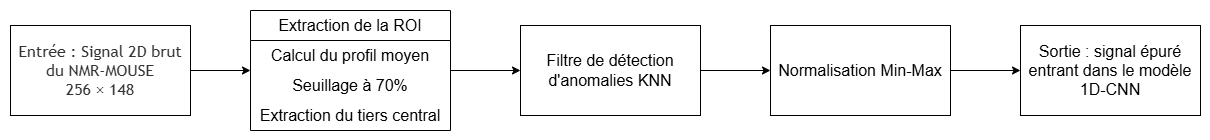
\includegraphics[width=0.9\textwidth]{pretraitement}
    \caption{chaîne totale du prétraitement des données de l'étude de \protect\cite{nuixe2024use}}
    \label{fig:pretraitement_chaine}
    \end{figure}


\subsection{Extraction de la ROI et réduction de dimensionnalité (2D vers 1D)}
\label{subsec:reduction_dimension}

Pour pallier le faible $SNR$ et éliminer les informations non pertinentes, une stratégie géométrique de réduction de dimension a été développée dans le module de traitement (synthétisée dans la Figure~\ref{fig:pretraitement_chaine}). Le signal 2D brut contient des couches de profondeur correspondant à des milieux extérieurs à la structure racinaire d'intérêt (air, vitre, terre pure). Le traitement applique les étapes suivantes :
\begin{enumerate}
    \item \textbf{Calcul du profil de densité moyen :} L'intensité moyenne du signal est calculée sur l'ensemble des profils temporels pour identifier la distribution spatiale de la matière (cf. Figure~\ref{fig:ROI_prof}).
    
\begin{figure}[htbp]
\centering
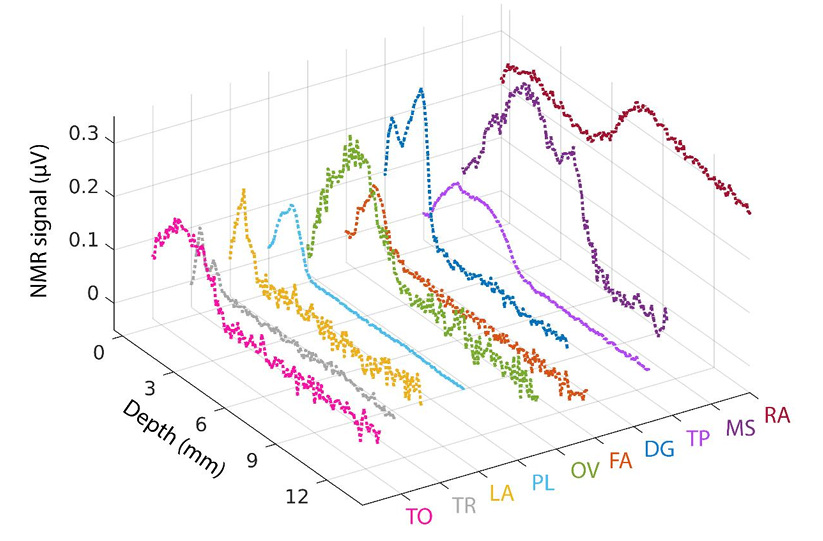
\includegraphics[width=0.8\textwidth]{Magali_ROI}
\caption{Intensité moyenne du signal de relaxation en fonction de la profondeur de mesure pour les 10 espèces du jeu de données \protect\cite{nuixe2024use}}
\label{fig:ROI_prof}
\end{figure}
    \item \textbf{Seuillage adaptatif :} Un seuil fixé à \num{70}\% de la valeur de crête du profil macroscopique isole les indices de profondeur correspondant au système racinaire.
    \item \textbf{Élimination des effets de bord :} Afin de se prémunir des artefacts de transition aux interfaces, le pipeline extrait le tiers central de la ROI détectée (sélection des canaux d'indice $\lfloor \frac{n}{3} \rfloor$ à $\lfloor \frac{2n}{3} \rfloor$). Une moyenne spatiale transforme ensuite la matrice 2D en un vecteur 1D de décroissance temporelle épuré.
\end{enumerate}

\subsection{Sélection empirique du modèle de détection d'anomalies}
\label{subsec:benchmark_outliers}

Le niveau de bruit du capteur, pouvant conduire à l'acquisition de signaux fortement dégradés, a rendu nécessaire l'intégration d'un module de détection d'anomalies en amont de la classification. La sélection de la méthode de détection n'a cependant pas pu être réalisée à partir de métriques supervisées classiques, telles que la précision, le rappel ou le score $F_1$, en l'absence d'un jeu de données annoté indiquant explicitement quels signaux devaient être considérés comme aberrants. La comparaison présentée dans cette section constitue donc une \textbf{sélection empirique}, fondée principalement sur la cohérence entre les anomalies détectées automatiquement et celles identifiées lors de l'inspection visuelle des signaux.

Afin de disposer d'un cas de référence suffisamment discriminant, nous avons d'abord isolé deux espèces, les espèces 3 et 5, pour lesquelles respectivement \num{16} et \num{51} mesures présentaient un profil particulièrement bruité et aberrant lors de l'analyse visuelle. La dégradation du rapport signal sur bruit ($SNR$) observée pour l'espèce 5 est notamment présentée en Figure~\ref{fig:SNR}. Ces observations ne constituent pas des annotations formelles, mais ont servi de \textbf{référence qualitative} pour comparer les différents algorithmes.

Six méthodes de détection d'anomalies disponibles dans la librairie \textit{PyOD} ont ainsi été évaluées : \textit{$K$-Nearest Neighbors} (KNN), \textit{Isolation Forest} (IForest), \textit{COPOD}, \textit{One-Class SVM} (OCSVM), \textit{HBOS} et \textit{PCA}. Pour chacune d'entre elles, nous avons comparé le nombre de mesures identifiées comme aberrantes avec les observations issues de l'analyse visuelle.

\begin{figure}[htbp]
\centering
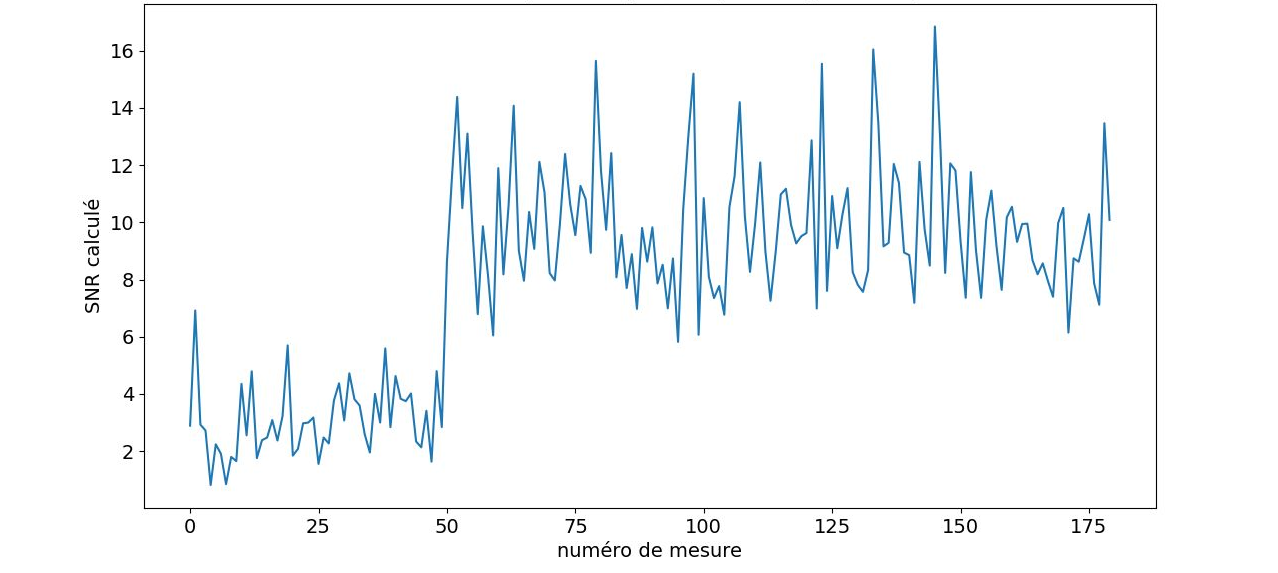
\includegraphics[width=0.8\textwidth]{SNR}
\caption{$SNR$ calculé pour le Medicago sativa (espèce 5), avec les 51 premières valeurs aberrantes}
\label{fig:SNR}
\end{figure}

\begin{table}[H]
\centering
\caption{Outliers détectés par espèce selon les méthodes de détection}
\label{tab:outliers_detection}
\resizebox{\textwidth}{!}{%
\begin{tabular}{|l|c|c|c|c|c|c|}
\hline
\textbf{Espèce} & \textbf{KNN} & \textbf{IForest} & \textbf{COPOD} & \textbf{OCSVM} & \textbf{HBOS} & \textbf{PCA} \
\hline
Espèce 1  & 2  & 6  & 2  & 6  & 2  & 4  \
\hline
Espèce 2  & 1  & 0  & 0  & 1  & 2  & 0  \
\hline
Espèce 3  & \cellcolor{green!30} 16 & 13 & 11 & 8  & \cellcolor{green!30} 16 & 8 \
\hline
Espèce 4  & 1  & 2  & 2  & 3  & 1  & 1  \
\hline
Espèce 5  & \cellcolor{green!30} 51 & 28 & 31 & 48 & 37 & 10 \
\hline
Espèce 6  & 2  & 2  & 2  & 2  & 1  & 2 \
\hline
Espèce 7  & 2  & 1  & 2  & 2  & 1  & 2 \
\hline
Espèce 8  & 0  & 0  & 0  & 0  & 0  & 0 \
\hline
Espèce 9  & 0  & 0  & 0  & 0  & 0  & 0 \
\hline
Espèce 10 & 0  & 0  & 0  & 0  & 0  & 0 \
\hline
\end{tabular}%
}
\end{table}

Les résultats mettent en évidence une différence notable entre les méthodes. Pour les deux espèces présentant les anomalies les plus visibles, KNN et HBOS détectent respectivement \num{16} et \num{51} observations pour l'espèce 3 et l'espèce 5, ce qui correspond exactement aux nombres de signaux identifiés visuellement comme aberrants. Les autres méthodes détectent un nombre différent d'observations sur au moins l'une de ces deux espèces. Cette concordance ne permet pas d'affirmer que les observations détectées par KNN constituent la totalité des anomalies présentes dans le jeu de données, mais elle fournit un \textbf{critère empirique de cohérence} en l'absence d'annotations de référence.

Le choix final du KNN repose ainsi sur la combinaison de deux critères pratiques. Premièrement, ses résultats sont cohérents avec les anomalies identifiées lors de l'inspection visuelle, en particulier pour les deux espèces les plus affectées. Deuxièmement, son temps d'exécution est inférieur à celui des autres méthodes testées, ce qui constitue un avantage dans le contexte d'un traitement appliqué systématiquement à l'ensemble des acquisitions. Le choix du KNN doit donc être interprété comme un \textbf{choix empirique adapté aux données disponibles et aux contraintes du pipeline}, et non comme la démonstration qu'il constitue intrinsèquement le meilleur algorithme de détection d'anomalies.

Le KNN a par conséquent été retenu pour le prétraitement des données et appliqué systématiquement avant l'étape de classification.


\section{Conception Logicielle et Pipeline d'Entraînement}
\label{sec:architecture_pipeline}

\subsection{Pipeline de données et labellisation physiologique}
\label{subsec:pipeline_data}

Les fenêtres temporelles de référence retenues au sein de la chambre climatique sont $[10\text{h}, 23\text{h}[$ pour la phase de jour et $[0\text{h}, 9\text{h}[$ pour la phase de nuit. Afin de tenir compte du temps de transition physiologique de la plante pour s'adapter au changement de son environnement, une portion de une heure a été exclue de mes données, après chaque basculement de cycle.

Le protocole de préparation des données intègre ensuite une normalisation par recentrage et réduction ($Z$-score global) appliquée à l'ensemble des échos ainsi qu'un partitionnement par validation croisée (\textit{$K$-Fold} avec $K=5$).

\subsection{Composants du réseau convolutif 1D-CNN}
\label{subsec:architecture_cnn}

L'architecture du modèle, nommée \textit{CNN1D\_multihead}, traite la nature séquentielle des \num{256} échos de relaxation. Elle repose sur l'enchaînement de trois couches de convolution monodimensionnelle, complétées par des mécanismes de stabilisation et de réduction de dimensionnalité :
\begin{itemize}
    \item \textbf{Batch Normalization 1D :} L'intégration de couches \textit{BatchNorm1d} après chaque bloc convolutif répond à une nécessité logique de stabilisation de l'apprentissage en maintenant une distribution homogène des activations au sein du réseau.
    \item \textbf{Adaptive Max Pooling 1D :} L'utilisation de la couche \textit{AdaptiveMaxPool1d} en sortie des blocs convolutifs permet de fixer une dimension de sortie constante pour la couche linéaire finale, indépendamment des variations de la taille des cartes de caractéristiques en amont.
\end{itemize}


\section{Résultats et Validation pour la classification jour-nuit}
\label{sec:resultats_analyse}
\subsection{Évaluation préliminaire par approche mono-espèce}
\label{subsec:approche_mono}

Afin de tester la faisabilité de notre classification et de valider l'hypothèse d'une signature circadienne propre à chaque entité biologique, une première campagne d'essais a été menée en isolant chaque espèce. Dix modèles \textit{1D-CNN} identiques ont été entraînés de manière totalement indépendante, chacun utilisant exclusivement les données d'une unique espèce (entraînement et validation en configuration intra-espèce). 

Cette approche quantitative permet d'établir une ligne de référence (\textit{baseline}) pour chaque dynamique racinaire et d'identifier le pouvoir discriminant intrinsèque de chaque signal, indépendamment de toute interférence globale. Les performances de cette étude de faisabilité sont répertoriées dans le tableau~\ref{tab:acc_mono_especes}.

\begin{table}[htbp]
\centering
\caption{Performances de faisabilité du modèle 1D-CNN entraîné et testé espèce par espèce}
\label{tab:acc_mono_especes}
\begin{tabular}{lccc}
\toprule
\textbf{Identifiant de l'Espèce} & \textbf{Accuracy Intra-Espèce} & \textbf{Volume de Test (Samples)} \\ 
\midrule
Espèce 1 & 91.4\% & 132 \\
Espèce 2 & 73.2\% & 140 \\
Espèce 3 & 59.3\% & 126 \\
Espèce 4 & 80.8\% & 128 \\
Espèce 5 & 61.2\% & 192 \\
Espèce 6 & 85.6\% & 140 \\
Espèce 7 & 63.5\% & 146 \\
Espèce 8 & 61.1\% & 132 \\
Espèce 9 & 77.3\% & 146 \\
Espèce 10 & 89.0\% & 174 \\ 
\bottomrule
\end{tabular}
\end{table}

Les résultats de ce tableau permettent de classifier immédiatement les espèces en deux catégories : celles présentant un taux de reconnaissance élevé (environ 80\%) et celles dont l'exactitude stagne plus proche du hasard (environ 60\%), confirmant une réponse plus faible au cycle jour/nuit sous les conditions du capteur pour ces espèces.

\subsection{Analyse comparative des performances : Noyau de référence vs Globalité des espèces}
\label{subsec:perf_especes}

L'analyse détaillée par entité biologique révèle des disparités de performance majeures et met en lumière l'impact de la variabilité inter-espèces sur la convergence du réseau. Pour évaluer la pertinence de notre ciblage, deux configurations d'entraînement ont été comparées.

Le tableau~\ref{tab:acc_4especes} présente les performances obtenues lorsque le modèle \textit{1D-CNN} est entraîné et validé uniquement sur le noyau de référence composé des 4 espèces les plus robustes face au bruit du capteur.

\begin{table}[htbp]
\centering
\caption{Performances d'exactitude du modèle 1D-CNN sur le noyau de référence (4 espèces clés)}
\label{tab:acc_4especes}
\begin{tabular}{lcc}
\toprule
\textbf{Identifiant de l'Espèce} & \textbf{Accuracy Globale} & \textbf{Volume de Test (Samples)} \\ 
\midrule
Espèce 1 & 86.92\% & 132 \\
Espèce 6 & 85.71\% & 140 \\
Espèce 9 & 75.82\% & 146 \\
Espèce 10 & 91.74\% & 174 \\ 
\bottomrule
\end{tabular}
\end{table}

À l'inverse, le tableau~\ref{tab:acc_10especes} expose les résultats d'un entraînement global centralisé englobant l'intégralité des 10 espèces du jeu de données initial, incluant donc les 6 espèces complexes ne discriminant pas clairement le jour de la nuit.

\begin{table}[htbp]
\centering
\caption{Performances du modèle 1D-CNN lors d'un entraînement global étendu aux 10 espèces}
\label{tab:acc_10especes}
\begin{tabular}{lcc}
\toprule
\textbf{Identifiant de l'Espèce} & \textbf{Accuracy Globale} & \textbf{Volume de Test (Samples)} \\ 
\midrule
Espèce 1 & 75.70\% & 132 \\
Espèce 2 & 67.05\% & 140 \\
Espèce 3 & 61.96\% & 126 \\
Espèce 4 & 58.24\% & 128 \\
Espèce 5 & 68.26\% & 192 \\
Espèce 6 & 79.12\% & 140 \\
Espèce 7 & 62.37\% & 146 \\
Espèce 8 & 60.55\% & 132 \\
Espèce 9 & 65.93\% & 146 \\
Espèce 10 & 88.99\% & 174 \\
\bottomrule
\end{tabular}
\end{table}

La comparaison de ces deux tableaux met en évidence le phénomène de perturbation de l'apprentissage global induit par les espèces non fonctionnelles. Lorsque l'entraînement intègre les 10 espèces, on observe une dégradation généralisée des scores d'exactitude, y compris sur des classes initialement stables (l'espèce 6.0 chute par exemple de \num{85.71}\% à \num{62.37}\%). 

Cette instabilité confirme que les signaux de ces 6 espèces agissent comme des perturbateurs lors de la rétropropagation, empêchant le classifieur d'établir une frontière de décision commune. Ces observations justifient empiriquement l'exclusion de ces données de la phase d'apprentissage centralisée et valident la nécessité de basculer vers une approche de fine-tuning ciblé ou une architecture multi-têtes.

\subsection{Analyse de la matrice de confusion}
\label{subsec:matrice_confusion}

Les résultats mettent en évidence un comportement équilibré du classifieur, le taux de faux positifs et le taux de faux négatifs restant proportionnels. Les erreurs résiduelles se concentrent majoritairement sur les points adjacents aux fenêtres de coupure temporelle, là où la réponse physiologique de la plante entame sa transition.

La matrice de confusion obtenue en cumulant les résultats de validation sur le noyau de référence (les 4 espèces clés) est présentée dans le tableau~\ref{tab:confusion_matrix}.

\begin{table}[htbp]
\centering
\caption{Matrice de confusion globale du modèle 1D-CNN (Classes : Jour et Nuit)}
\label{tab:confusion_matrix}
\vspace{0.3cm}
\begin{tabular}{l|cc}
\toprule
\textbf{Réel $\backslash$ Prédit} & \textbf{Jour} & \textbf{Nuit} \\ 
\midrule
\textbf{Jour} & \textbf{213} & 22 \\
\textbf{Nuit} & 36 & \textbf{127} \\
\bottomrule
\end{tabular}
\end{table}

L'analyse de cette matrice permet d'extraire les métriques secondaires suivantes :
\begin{itemize}
    \item \textbf{Rappel (Recall) pour la classe Jour :} \num{90.64}\% (\num{213} sur \num{235} échantillons réels).
    \item \textbf{Rappel (Recall) pour la classe Nuit :} \num{77.91}\% (\num{127} sur \num{163} échantillons réels).
    \item \textbf{Précision globale :} \num{85.42}\% pour le Jour et \num{85.23}\% pour la Nuit.
\end{itemize}
Cette asymétrie de sensibilité (\num{90.64}\% vs \num{77.91}\%) confirme que les signaux nocturnes sont légèrement plus difficiles à classifier.


\subsection{Explicabilité du modèle par approche Grad-CAM et pertinence biophysique}
\label{subsec:explicabilite_resultats}

Conformément aux objectifs scientifiques fixés, une étude d'explicabilité a été menée pour analyser les prédictions unitaires du modèle \textit{1D-CNN}. Pour ce faire, l'algorithme \textit{Grad-CAM} (\textit{Gradient-weighted Class Activation Mapping}) a été adapté et implémenté sur notre architecture convolutive monodimensionnelle. En utilisant les gradients du score de la classe prédite relativement aux cartes de caractéristiques (\textit{feature maps}) de la dernière couche convolutive, Grad-CAM permet de calculer un vecteur d'importance grossier qui est ensuite moyenné sur des portions de 32 points de large.


Les cartes Grad-CAM obtenues pour les différentes espèces ont été regroupées selon leurs performances de classification et leur comportement observé. Trois catégories ont ainsi été identifiées : les espèces de référence, les espèces présentant une accuracy proche de 60\,\% et les autres espèces.

\subsubsection{Espèces de référence}

Cette première catégorie regroupe les quatre espèces de référence utilisées dans l'étude. Les profils d'importance présentés sur la Figure~\ref{fig:gradcam_reference} permettent d'identifier les régions du signal principalement exploitées par le modèle pour réaliser la classification.

\begin{figure}[htbp]
    \centering
    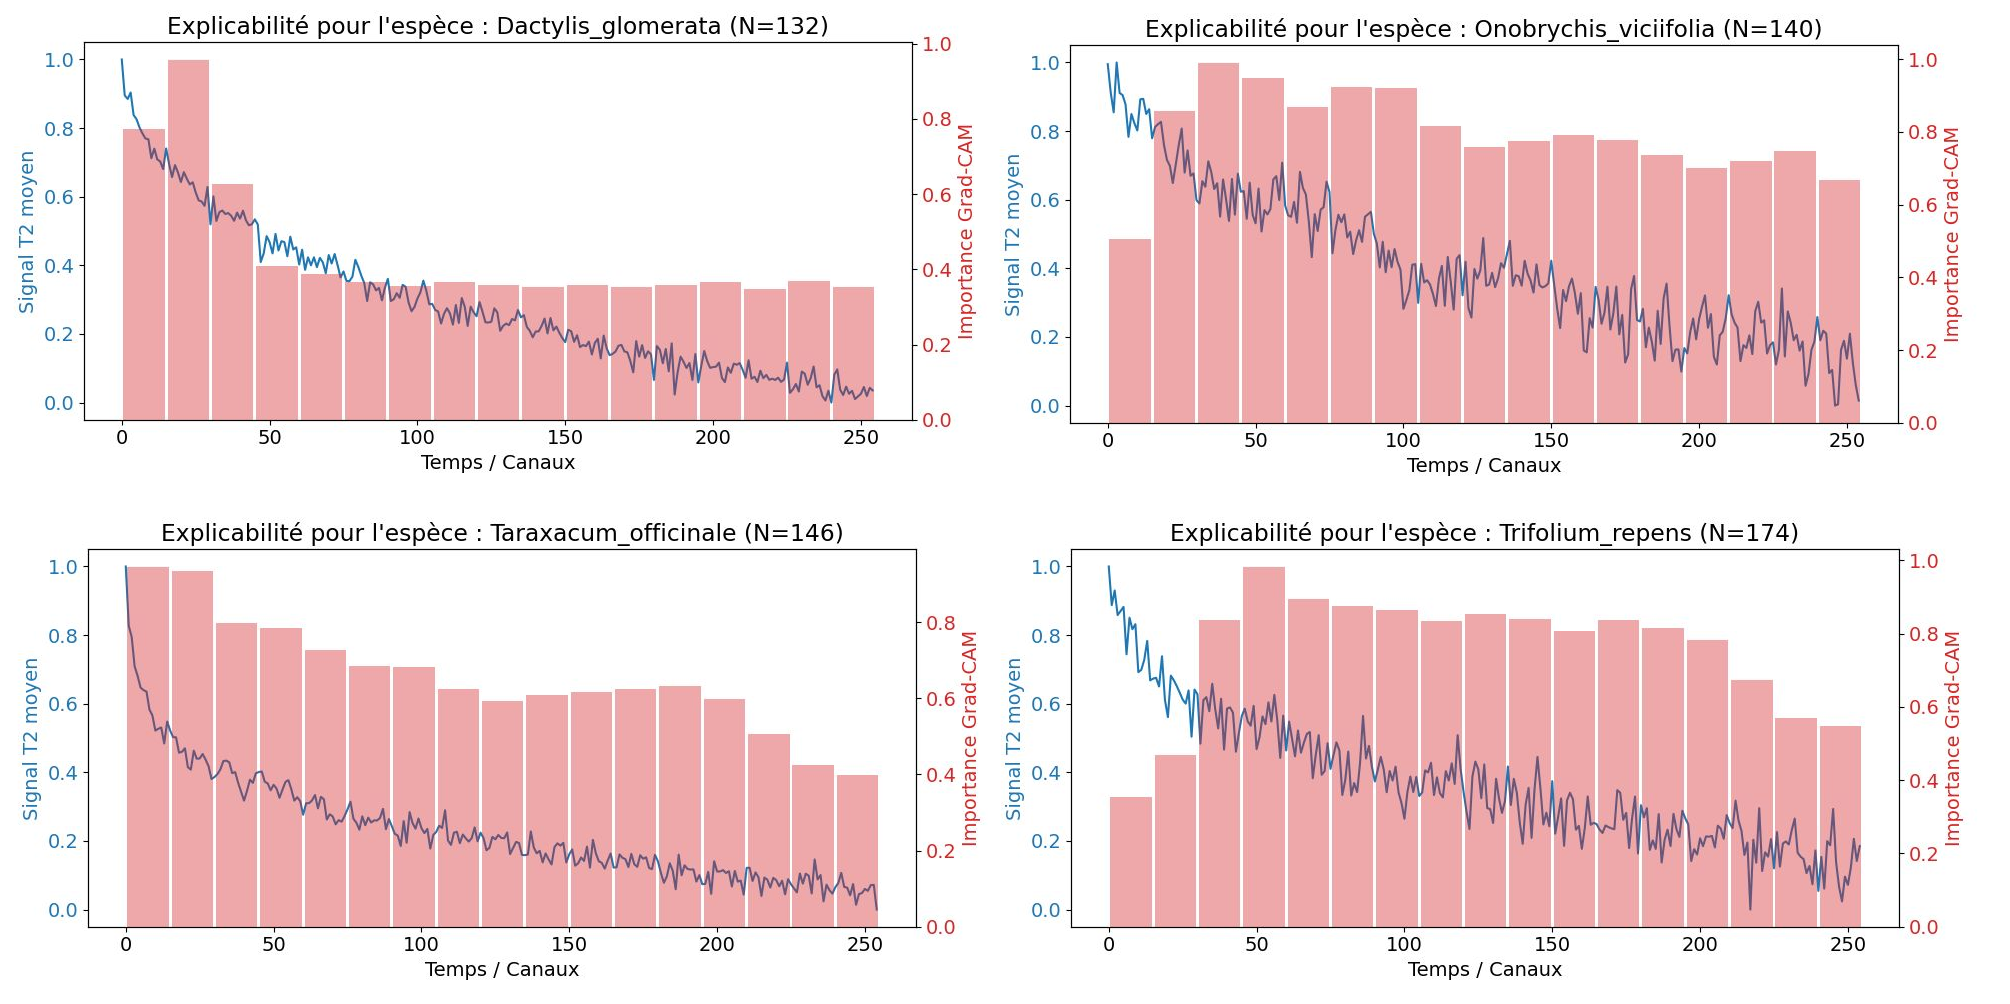
\includegraphics[width=\textwidth]{grad-ref}
    \caption{Cartes Grad-CAM moyennes des 4 espèces de référence.}
    \label{fig:gradcam_reference}
\end{figure}

\subsubsection{Espèces présentant une accuracy proche de 60\,\%}

Cette catégorie regroupe les deux espèces pour lesquelles les performances de classification sont les plus faibles, avec une accuracy d'environ 60\,\%. L'analyse des cartes Grad-CAM illustrées sur la Figure~\ref{fig:gradcam_60acc} permet d'étudier les zones du signal utilisées par le modèle et d'identifier d'éventuelles causes de confusion entre les classes.

\begin{figure}[htbp]
    \centering
    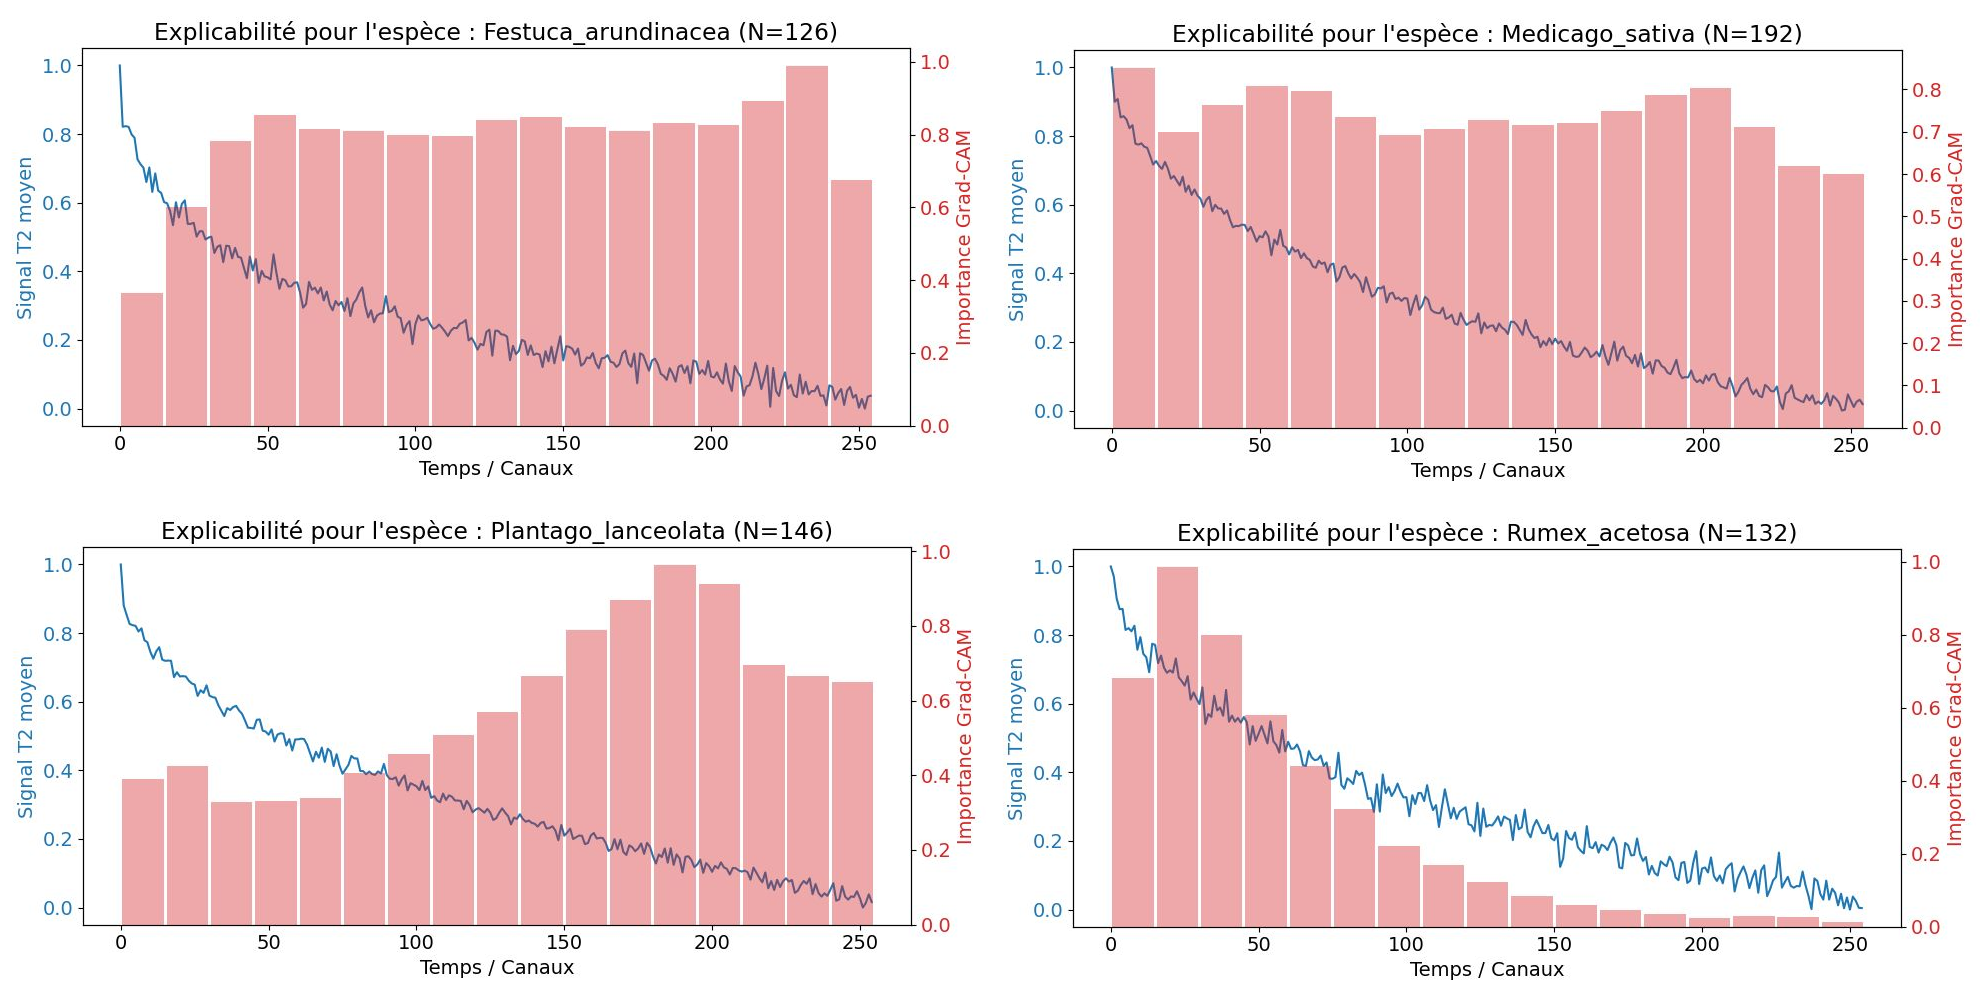
\includegraphics[width=\textwidth]{60}
    \caption{Cartes Grad-CAM moyennes des espèces présentant une accuracy proche de 60\,\%.}
    \label{fig:gradcam_60acc}
\end{figure}

\subsubsection{Autres espèces}

Enfin, cette dernière catégorie regroupe les deux espèces restantes. Celles-ci présentent la particularité d'être correctement discriminées lors d'un apprentissage dédié (intra-espèce), mais s'avèrent incapables de converger au sein d'un modèle global, leur signal entrant en conflit avec la dynamique générale du jeu de données. Leurs profil d'activation Grad-CAM sont représentés en Figure~\ref{fig:gradcam_autres}.

\begin{figure}[htbp]
    \centering
    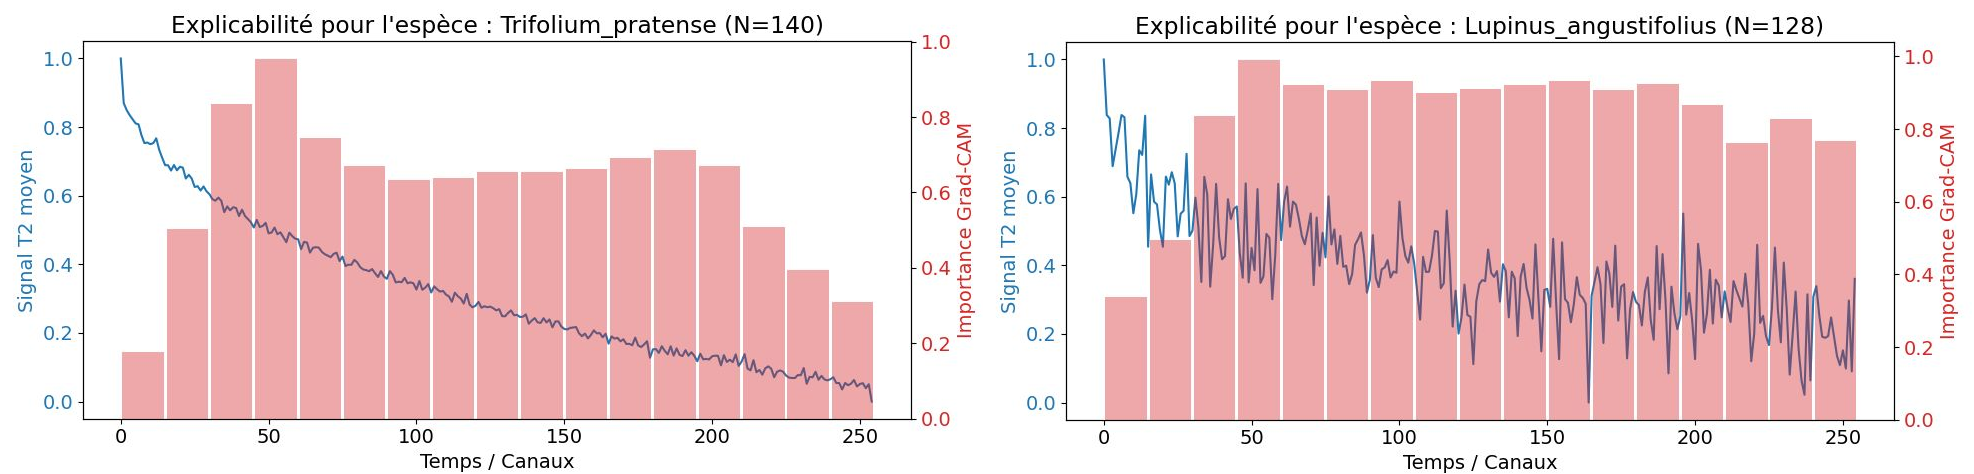
\includegraphics[width=\textwidth]{autres}
    \caption{Cartes Grad-CAM moyennes des autres espèces étudiées.}
    \label{fig:gradcam_autres}
\end{figure}

\subsubsection{Discussion}

 En l'état actuel des travaux, l'interprétation exhaustive de ces courbes d'explicabilité reste limitée. Cependant, les avancées conjointes menées au sein de l'équipe sur la simulation de signaux RMN en fonction de la physiologie racinaire ouvrent une perspective prometteuse. Entraîner le modèle sur ces données simulées, bénéficiant d'un rapport signal sur bruit ($SNR$) idéal, permettrait de générer des courbes d'explicabilité de référence. La comparaison de nos résultats à cette base théorique parfaite offrirait ainsi un point de comparaison rigoureux pour valider la pertinence physique des motifs extraits par le réseau.



\section{Exploitation des données RMN simulées}
\label{sec:simul}

\subsection{Objectif de l'étude}
\label{subsec:obj_simul}

L'utilisation de données simulées constitue une approche complémentaire aux données expérimentales afin d'évaluer la quantité d'information physiologique effectivement contenue dans les signaux RMN. L'objectif de cette étude est de répondre à la question suivante :

\begin{quote}
\textit{Une simulation des signaux RMN permet-elle, à elle seule, d'obtenir des performances de classification acceptables, ou l'utilisation de données expérimentales reste-t-elle indispensable ?}
\end{quote}

Cette question présente un double intérêt. D'une part, des données simulées permettent de contrôler précisément les paramètres physiques intervenant dans la génération du signal et de produire un volume important de données sans nécessiter de nouvelles acquisitions expérimentales. D'autre part, elles constituent un environnement simplifié dans lequel le réseau de neurones peut apprendre des relations entre les paramètres simulés et l'état physiologique sans être directement confronté à l'ensemble des perturbations présentes dans les acquisitions réelles.

L'étude a donc été menée selon une stratégie de pré-entraînement sur les données simulées, suivie de plusieurs protocoles permettant d'évaluer la capacité de généralisation du modèle vers les données expérimentales.

\subsection{Pré-entraînement sur les données simulées}
\label{subsec:pretrain_simul}

Dans un premier temps, le modèle convolutif est entraîné exclusivement sur les signaux générés par simulation. L'objectif est de déterminer si les caractéristiques apprises à partir de ces données sont directement exploitables sur les signaux expérimentaux.

Le modèle utilisé repose sur la même architecture convolutive que celle employée pour l'analyse des données expérimentales. Cette approche permet de comparer les différents protocoles de transfert sans introduire de différence liée à l'architecture du réseau.

Le pré-entraînement consiste à optimiser l'ensemble des paramètres du réseau sur les données simulées. Une fois cette étape réalisée, les poids obtenus sont utilisés comme point de départ pour les différentes stratégies de transfert étudiées.

\subsection{Évaluation du transfert vers les données expérimentales}
\label{subsec:eval_transfert}

Trois stratégies ont été comparées afin d'évaluer le degré de transférabilité des représentations apprises sur les données simulées :

\begin{enumerate}
\item \textbf{Zero-shot :} les poids obtenus lors du pré-entraînement sont directement utilisés sur les données expérimentales, sans aucune phase d'apprentissage supplémentaire ;

\item \textbf{Transfer learning avec backbone gelé :} les couches convolutives apprises sur les données simulées sont conservées et leurs paramètres sont gelés. Seule la partie de classification est ré-entraînée à partir des données expérimentales ;

\item \textbf{Fine-tuning :} les poids issus du pré-entraînement sont utilisés comme initialisation, mais l'ensemble du réseau reste entraînable lors de l'apprentissage sur les données expérimentales.

\end{enumerate}

Cette comparaison permet de distinguer deux effets. Le premier est la capacité intrinsèque des représentations apprises sur simulation à se généraliser à des données qui n'ont jamais été observées pendant l'entraînement. Le second correspond à la capacité du réseau à adapter ces représentations aux spécificités des acquisitions expérimentales.

\subsection{Résultats}
\label{subsec:res_simul}

Les résultats obtenus montrent que les données simulées contiennent bien une information exploitable pour la classification. En particulier, l'approche \textit{zero-shot} permet d'obtenir une accuracy d'environ \num{60}\%, avec certaines espèces atteignant environ \num{70}\%. Ces performances sont supérieures à un comportement purement aléatoire, mais restent éloignées des performances obtenues lorsque le modèle est entraîné directement sur les données expérimentales.

Le résultat obtenu en \textit{zero-shot} constitue ainsi un premier élément en faveur de l'existence d'une information commune entre les signaux simulés et expérimentaux. Le réseau est capable de produire des prédictions pertinentes sur des signaux qu'il n'a jamais utilisés pour son apprentissage. Cependant, le niveau de performance obtenu reste insuffisant pour considérer la simulation seule comme une solution complète au problème de classification.

Les stratégies intégrant une phase d'apprentissage sur les données expérimentales permettent d'améliorer ces performances. Les meilleurs résultats sont obtenus lorsque le \textbf{backbone convolutif n'est pas gelé}. Le fine-tuning de l'ensemble du réseau permet ainsi d'adapter les représentations apprises sur les signaux simulés aux caractéristiques spécifiques des mesures expérimentales.
\begin{table}[htbp]
\centering
\caption{Comparaison des stratégies de transfert entre données simulées et expérimentales.}
\label{tab:transfer}
\begin{tabular}{lcc}
\toprule
\textbf{Stratégie} & \textbf{Backbone} & \textbf{Accuracy} \\
\midrule
Zero-shot       & Gelé      & $58\% \pm 1\%$ \\
Transfer learning & Gelé    & $64\% \pm 2\%$ \\
Fine-tuning     & Non gelé  & $75\% \pm 2\%$ \\
\bottomrule
\end{tabular}
\end{table}

Ces résultats mettent en évidence une limite importante du transfert direct entre simulation et expérimentation. Les représentations apprises à partir des données simulées sont suffisamment pertinentes pour extraire une partie de l'information discriminante présente dans les signaux réels, mais elles ne permettent pas de reproduire intégralement la complexité des acquisitions expérimentales.

\subsection{Limites de la simulation}
\label{subsec:limites_simul}

Une première limite de l'approche réside dans le nombre de paramètres physiques pris en compte lors de la génération des signaux simulés. La simulation ne reproduit pas nécessairement l'ensemble des facteurs susceptibles d'influencer les acquisitions expérimentales. Certains paramètres pouvant modifier la forme ou l'amplitude du signal ne sont ainsi pas représentés dans le modèle de simulation.

La température constitue notamment un exemple important. Les conditions expérimentales sont contrôlées par des chambres climatiques, avec une température d'environ \SI{18}{\degreeCelsius} durant la journée et \SI{21}{\degreeCelsius} durant la nuit. Cette faible plage de variation limite cependant la possibilité d'étudier expérimentalement l'influence indépendante de la température sur le signal : celle-ci varie principalement avec le cycle jour/nuit et ne peut donc pas être facilement dissociée de l'état physiologique étudié.

Cette contrainte expérimentale constitue une difficulté pour enrichir directement le modèle de simulation à partir des observations réelles. Il est en effet difficile d'estimer séparément l'effet de la température et celui du cycle physiologique lorsque ces deux variables évoluent de manière fortement corrélée dans le protocole expérimental.

Ainsi, les performances obtenues en \textit{zero-shot} montrent que la simulation reproduit une partie des caractéristiques pertinentes des signaux expérimentaux, mais les écarts observés après transfert suggèrent que certains facteurs absents de la simulation restent nécessaires pour reproduire fidèlement les données réelles.

\subsection{Discussion}
\label{subsec:discussion_simul}

L'expérience permet finalement de répondre partiellement à la question initiale. La simulation seule ne permet pas d'obtenir les meilleures performances de classification, mais elle n'est pas non plus dépourvue de pouvoir discriminant. Les performances obtenues en \textit{zero-shot}, supérieures au hasard et pouvant atteindre environ \num{70}\% selon les espèces, montrent que le réseau apprend des représentations qui conservent une partie de l'information pertinente lors du passage des données simulées aux données expérimentales.

L'amélioration obtenue lorsque le backbone est laissé entraînable est particulièrement informative. Elle suggère que les caractéristiques générales apprises sur les simulations constituent une bonne initialisation, mais qu'elles doivent être adaptées aux spécificités des acquisitions réelles. Le fine-tuning permet ainsi de conserver une partie des connaissances acquises lors du pré-entraînement tout en ajustant les représentations aux phénomènes non reproduits par la simulation.

La simulation apparaît donc davantage comme un \textbf{outil de pré-entraînement et d'analyse} que comme un substitut complet aux données expérimentales. Elle pourrait notamment permettre de générer de grandes quantités de données contrôlées, d'étudier l'influence de paramètres physiques difficilement isolables expérimentalement et de fournir une référence pour l'interprétation des caractéristiques apprises par le réseau.

\section{Exploitation de la dimension spatiale des signaux RMN}
\label{sec:signaux_2d}

\subsection{Contexte et objectif}
\label{subsec:contexte_2d}

Une seconde partie du travail a consisté à étudier des signaux RMN acquis sur des troncs d'arbres dans le cadre d'une expérimentation sur le stress hydrique. Cette expérimentation diffère des données précédemment étudiées, notamment par l'importance de la dimension spatiale du signal.

Cinq arbres ont été suivis quotidiennement au cours de l'expérimentation. Deux arbres ont été maintenus dans des conditions témoins, avec un apport en eau continu, tandis que trois arbres ont été progressivement soumis à un assèchement volontaire afin de provoquer un stress hydrique. Les signaux obtenus sont constitués d'une matrice bidimensionnelle de taille $512 \times 128$. La première dimension correspond à l'évolution temporelle du signal RMN, tandis que la seconde correspond à la dimension spatiale, associée aux différentes profondeurs du tronc.

Dans ce contexte, la réduction des signaux à une seule dimension, utilisée précédemment pour les données étudiées sur les racines, risque de supprimer une partie de l'information pertinente. En effet, les propriétés du tronc peuvent varier selon sa profondeur, et l'effet du stress hydrique peut donc se manifester différemment dans les différentes couches de l'arbre.

L'objectif de cette étude est ainsi d'évaluer si l'exploitation directe de la matrice $2D$ permet au réseau de neurones de tirer parti de cette information spatiale pour distinguer les arbres stressés des arbres témoins.

\subsection{Jeu de données}
\label{subsec:dataset_2d}

Le jeu de données est constitué de mesures réalisées quotidiennement sur cinq arbres. Deux arbres constituent le groupe témoin et sont arrosés continuellement au cours de l'expérimentation, tandis que trois arbres sont soumis à une période d'assèchement volontaire.

Le problème de classification comporte deux classes correspondant aux états \textit{stressé} et \textit{non stressé}. Chaque mesure est représentée par une matrice de taille $512 \times 128$. Contrairement à l'approche précédente, aucune réduction de la dimension spatiale n'est effectuée avant l'entrée dans le réseau : l'ensemble de la structure bidimensionnelle du signal est conservé.

Cette représentation permet au modèle d'exploiter simultanément l'évolution temporelle du signal et sa variation selon la profondeur du tronc.

\subsection{Architecture du réseau convolutif 2D}
\label{subsec:cnn_2d}

Afin d'exploiter directement la structure spatiale des signaux, un réseau de neurones convolutif bidimensionnel (\textit{Convolutional Neural Network}, CNN) a été développé.

L'architecture est composée de trois couches de convolution $2D$, chacune suivie d'une normalisation par lots (\textit{Batch Normalization}) et d'une fonction d'activation ReLU. Les convolutions utilisent un stride de $2$ afin de réduire progressivement les dimensions spatiales de la représentation tout en augmentant le nombre de caractéristiques extraites.

À l'issue des trois blocs convolutifs, un \textit{Adaptive Average Pooling} ou \textit{Adaptive Max Pooling} est utilisé afin de ramener la représentation à une taille fixée indépendamment des dimensions intermédiaires. La représentation obtenue est ensuite aplatie puis transmise à deux couches entièrement connectées, de tailles respectives $128$ et $32$ neurones. Une dernière couche entièrement connectée produit les deux scores correspondant aux deux classes.

La structure générale du réseau est donc la suivante :

\begin{center}
\begin{verbatim}
Signal 2D (512 x 128)
        |
        v
Conv2D + BatchNorm + ReLU
        |
        v
Conv2D + BatchNorm + ReLU
        |
        v
Conv2D + BatchNorm + ReLU
        |
        v
Adaptive Pooling
        |
        v
Fully Connected (128)
        |
        v
Fully Connected (32)
        |
        v
Classification (2 classes)
\end{verbatim}
\end{center}

Un mécanisme de dropout est également utilisé dans les couches entièrement connectées afin de limiter le surapprentissage.

\subsection{Optimisation des hyperparamètres}
\label{subsec:optimisation_2d}

L'architecture et les hyperparamètres du réseau ont été déterminés à l'aide de la méthode d'optimisation bayésienne présentée précédemment. Cette optimisation permet de rechercher automatiquement une configuration adaptée aux données plutôt que de fixer manuellement l'ensemble des paramètres du réseau.

Les paramètres explorés comprennent notamment le nombre de filtres des différentes couches convolutives, les tailles des noyaux, le taux de dropout, la taille des couches entièrement connectées, la taille du pooling ainsi que les paramètres d'apprentissage.

La meilleure configuration obtenue lors de cette recherche correspond à une accuracy de validation de $88\%$ au cours du processus d'optimisation. La configuration retenue est présentée dans le tableau~\ref{tab:best_config_2d}.

\begin{table}[htbp]
    \centering
    \caption{Configuration optimale obtenue par optimisation bayésienne pour le CNN 2D.}
    \label{tab:best_config_2d}
    \begin{tabular}{lc}
        \toprule
        \textbf{Hyperparamètre} & \textbf{Valeur} \\
        \midrule
        Nombre de filtres, couche 1 & 32 \\
        Nombre de filtres, couche 2 & 4 \\
        Nombre de filtres, couche 3 & 64 \\
        Taille de la couche FC 1 & 128 \\
        Taille de la couche FC 2 & 32 \\
        Taille du pooling & $64$ \\
        Taux de dropout & $0.128$ \\
        Learning rate & $0.00220$ \\
        Weight decay & $1.07\times10^{-6}$ \\
        \bottomrule
    \end{tabular}
\end{table}

\subsection{Évaluation du modèle}
\label{subsec:evaluation_2d}

Les performances finales du modèle ont été évaluées à l'aide d'une validation croisée stratifiée en cinq plis (\textit{Stratified K-Fold Cross Validation}). Les mesures provenant des différents arbres sont regroupées dans le jeu de données avant la réalisation de la séparation en cinq plis.

Les accuracies obtenues pour les cinq plis sont respectivement de $85\%$, $80\%$, $80\%$, $85\%$ et $85\%$. La moyenne obtenue est donc de $83.0\%$, avec un écart-type de $2.4$ points de pourcentage.

\begin{table}[htbp]
    \centering
    \caption{Accuracy obtenue pour les cinq plis de validation croisée.}
    \label{tab:results_2d}
    \begin{tabular}{lc}
        \toprule
        \textbf{Fold} & \textbf{Accuracy} \\
        \midrule
        1 & $85\%$ \\
        2 & $80\%$ \\
        3 & $80\%$ \\
        4 & $85\%$ \\
        5 & $85\%$ \\
        \midrule
        Moyenne & $\mathbf{83.0\%}$ \\
        Écart-type & $\mathbf{2.4}$ points \\
        \bottomrule
    \end{tabular}
\end{table}

La faible dispersion des performances entre les différents plis indique une certaine stabilité du modèle sur le jeu de données considéré. Les performances obtenues montrent ainsi qu'un modèle convolutif exploitant directement la représentation bidimensionnelle des signaux est capable de distinguer les deux états physiologiques avec une accuracy moyenne de l'ordre de $83\%$.

Il convient cependant de noter que la séparation des données a été réalisée au niveau des mesures et non au niveau des arbres. Les différents plis peuvent donc contenir des mesures provenant d'un même arbre. Les performances obtenues caractérisent ainsi principalement la capacité du modèle à généraliser à de nouvelles mesures issues des arbres observés, et ne permettent pas à elles seules d'évaluer sa capacité à généraliser à un arbre totalement nouveau.

\subsection{Limites du protocole de validation croisée}
\label{subsec:limites_kfold_2d}

La validation croisée présentée précédemment est réalisée au niveau des mesures et non au niveau des individus. Ainsi, plusieurs acquisitions provenant d'un même arbre peuvent être présentes simultanément dans les ensembles d'entraînement et de validation. Ce choix doit être pris en compte dans l'interprétation des performances obtenues.

Le nombre limité d'individus disponibles, soit cinq arbres au total, ne permet pas de réaliser une évaluation robuste de la généralisation inter-individus. Une séparation stricte des données au niveau des arbres aurait conduit à des ensembles de validation constitués d'un nombre très faible d'individus. Cette difficulté est particulièrement importante pour la classe témoin, qui ne comporte que deux arbres. Dans ces conditions, les performances mesurées auraient été fortement dépendantes de l'individu sélectionné pour la validation et auraient fourni une estimation peu robuste de la performance du modèle.

La validation croisée a donc été réalisée au niveau des mesures afin d'évaluer, dans un premier temps, la capacité du modèle à classifier de nouvelles acquisitions provenant des individus observés. Ce protocole permet d'exploiter l'ensemble des mesures disponibles tout en conservant une stratification entre les deux classes.

Cette stratégie présente néanmoins une limite importante. Les mesures successives provenant d'un même arbre peuvent être corrélées et partager certaines caractéristiques propres à cet individu. La présence de mesures d'un même arbre dans les ensembles d'entraînement et de validation peut ainsi conduire le réseau à exploiter indirectement une information liée à l'identité de l'arbre plutôt qu'à la seule signature du stress hydrique. Les performances obtenues peuvent par conséquent être optimistes par rapport à celles qui seraient observées sur un arbre totalement nouveau.

Les résultats doivent donc être interprétés comme une \textbf{évaluation de la généralisation à de nouvelles mesures issues des individus étudiés}, et non comme une démonstration de la généralisation à de nouveaux individus.

Une validation plus stricte, fondée par exemple sur une séparation groupée par arbre (\textit{Group K-Fold} ou \textit{Leave-One-Tree-Out}), constituerait une évaluation plus pertinente de la généralisation inter-individus. Cependant, sa fiabilité nécessiterait un nombre d'arbres sensiblement plus important, notamment pour disposer d'un nombre suffisant d'individus dans chacune des classes. L'acquisition de données supplémentaires sur un plus grand nombre d'arbres permettrait ainsi, à terme, de mettre en place un protocole de validation indépendant de l'identité individuelle.

\subsection{Apport de la représentation bidimensionnelle pour l'explicabilité}
\label{subsec:gradcam_2d}

L'utilisation d'une architecture convolutive $2D$ présente également un intérêt important pour l'interprétation des décisions du modèle. Une méthode Grad-CAM++ a été appliquée aux couches convolutives du réseau afin d'identifier les régions du signal contribuant le plus à la classification.

Contrairement à l'approche utilisée pour les signaux unidimensionnels, l'explicabilité est ici naturellement représentée sous la forme d'une carte bidimensionnelle. Pour chaque signal, trois représentations peuvent être comparées : le signal RMN original, la carte d'importance obtenue par Grad-CAM++ et la superposition de cette carte sur le signal original.

Les résultats montrent que le réseau ne répartit pas uniformément son attention sur l'ensemble du signal. Une importance particulièrement élevée apparaît dans certaines régions correspondant à des zones spécifiques de la représentation temporelle et spatiale, comme illustré pour la classe stressée dans la Figure~\ref{fig:gradcam_2d_stress}. Cette information est difficile à conserver lorsqu'une matrice $2D$ est réduite à une seule courbe.

\begin{figure}[htbp]
    \centering
    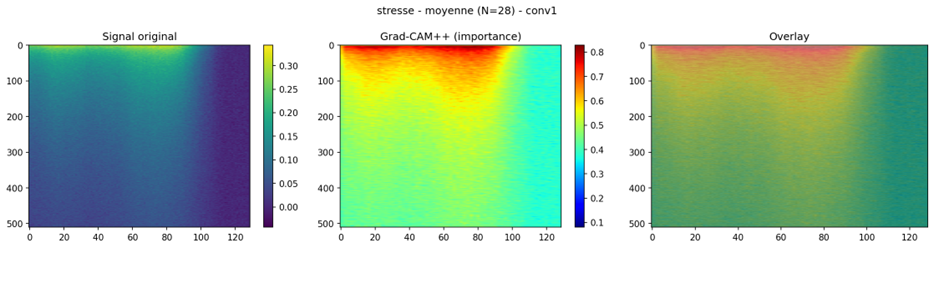
\includegraphics[width=\textwidth]{gradcam_2d_stress.png}
    \caption{Exemple de cartes Grad-CAM++ obtenues pour les signaux de la classe stressée. De gauche à droite : signal RMN original, carte d'importance et superposition de la carte sur le signal.}
    \label{fig:gradcam_2d_stress}
\end{figure}

Une observation similaire peut être réalisée pour les signaux correspondant aux arbres non stressés (Figure~\ref{fig:gradcam_2d_control}). Les cartes mettent en évidence des régions différentes selon la classe prédite, ce qui suggère que le réseau exploite des caractéristiques localisées dans la représentation spatio-temporelle du signal.

\begin{figure}[htbp]
    \centering
    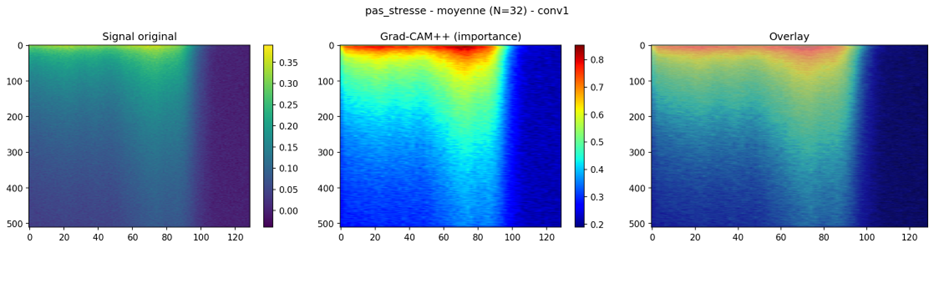
\includegraphics[width=\textwidth]{gradcam_2d_control.png}
    \caption{Exemple de cartes Grad-CAM++ obtenues pour les signaux de la classe non stressée. De gauche à droite : signal RMN original, carte d'importance et superposition de la carte sur le signal.}
    \label{fig:gradcam_2d_control}
\end{figure}

L'utilisation d'une carte d'importance permet également d'aller au-delà d'une simple visualisation de la zone sélectionnée par le réseau. Les régions identifiées comme importantes peuvent être utilisées pour retrouver les signaux de relaxation correspondants et les représenter sous forme de courbes. Cette étape permet ainsi de relier l'explication fournie par le réseau à une représentation physique plus directement interprétable du signal RMN.

\subsection{Discussion}
\label{subsec:discussion_2d}

Cette expérience montre l'intérêt de conserver la dimension spatiale des signaux dans le cas de mesures réalisées sur les troncs. Alors que la réduction des signaux $2D$ vers une représentation $1D$ constituait une étape utile pour les données précédemment étudiées, elle pourrait ici conduire à une perte d'information discriminante.

Le modèle $2D$ obtient une accuracy moyenne de $83.0\% \pm 2.4\%$ sur les cinq plis de validation croisée. Ces résultats montrent qu'il est possible d'exploiter directement la structure spatio-temporelle des signaux pour distinguer les arbres soumis à un stress hydrique des arbres témoins.

L'intérêt de cette représentation ne se limite cependant pas aux performances de classification. Les cartes Grad-CAM++ présentées aux Figures~\ref{fig:gradcam_2d_stress} et \ref{fig:gradcam_2d_control} fournissent une localisation spatiale des régions utilisées par le réseau pour prendre sa décision. Elles permettent ainsi d'identifier simultanément les zones temporelles et les profondeurs du tronc auxquelles le modèle accorde le plus d'importance.

Cette information constitue un avantage important par rapport à une représentation purement unidimensionnelle. Elle ouvre notamment la possibilité d'étudier si les caractéristiques discriminantes sont localisées dans certaines couches du tronc et si leur localisation évolue au cours du développement du stress hydrique.

Il reste néanmoins nécessaire d'interpréter ces cartes avec prudence. Une zone fortement activée par Grad-CAM++ indique qu'elle contribue à la décision du réseau, mais ne constitue pas à elle seule une preuve de l'existence d'un mécanisme biologique causal. Une analyse complémentaire des signaux correspondant aux régions identifiées est donc nécessaire pour relier les caractéristiques apprises par le modèle aux phénomènes physiques et physiologiques sous-jacents.
\section{Discussion générale}
\label{sec:discussion}

\subsection{Retour d'expérience}

Ce projet a permis de confronter les méthodes d'apprentissage profond à une
problématique où la performance algorithmique ne peut être dissociée de la
qualité des acquisitions et de leur interprétation physique. La mise en place
du pipeline a notamment montré l'importance du prétraitement et de la
caractérisation des données avant toute étape d'apprentissage.

Le travail sur l'explicabilité a également mis en évidence une différence
importante entre l'obtention d'une bonne performance de classification et la
compréhension du comportement du modèle. Dans le contexte de données
biologiques, cette seconde dimension est essentielle afin de distinguer une
information physiologique pertinente d'un artefact propre aux acquisitions ou
au jeu de données.

Cette expérience a ainsi permis de développer une approche plus globale de la
conception de modèles d'apprentissage automatique, intégrant à la fois la
qualité des données, le choix du modèle, son optimisation, son évaluation et
l'interprétation de ses prédictions.

\section{Responsabilité sociétale et environnementale}
\label{sec:rse}

Cette partie présente une analyse des impacts environnementaux et sociétaux associés au projet de fin d'études. Conformément aux recommandations de l'ENSIMAG, l'analyse est structurée selon trois niveaux : l'impact environnemental direct lié à la réalisation du PFE, l'impact environnemental et sociétal global du projet, puis la politique de responsabilité sociétale et environnementale de la structure d'accueil.

L'objectif n'est pas de réaliser une analyse de cycle de vie exhaustive du projet, ce qui nécessiterait des données et des moyens qui dépassent le cadre de ce travail, mais d'identifier les principaux postes d'impact, d'en estimer les ordres de grandeur et d'en discuter les principales limites.

\subsection{Impact environnemental personnel du PFE}
\label{subsec:rse_impact_personnel}

La réalisation de ce PFE a généré plusieurs types d'impacts environnementaux directs : les déplacements domicile-travail, l'utilisation du matériel informatique mis à disposition et l'utilisation de ressources de calcul, notamment des GPU. Afin de comparer ces différents postes, les consommations énergétiques sont, lorsque cela est possible, converties en potentiel de réchauffement climatique exprimé en kilogrammes équivalent CO$_2$ (kg CO$_2$e).

Les estimations présentées ci-dessous reposent sur des hypothèses simplificatrices et doivent donc être interprétées comme des ordres de grandeur. En particulier, l'empreinte liée à la fabrication des équipements ne peut pas être attribuée précisément à un seul projet lorsque ceux-ci existaient déjà avant le début du PFE et sont utilisés successivement par plusieurs personnes.

\subsubsection{Impact des trajets domicile-travail}
\label{subsubsec:rse_transport}

Le PFE s'est déroulé sur une durée de 23 semaines. En considérant une présence moyenne de cinq jours par semaine, cela correspond à environ 115 journées de travail.

Le trajet quotidien entre le domicile et le lieu de travail représente environ 18 km dans un seul sens, soit 36 km par journée de travail. Le trajet est effectué en transports en commun, avec une première partie d'environ 5 km en tramway, puis le reste en bus.

Sur l'ensemble de la période, la distance parcourue peut donc être estimée à :

$$
115 \times 36 = 4140\ \text{km}.
$$

Le recours aux transports collectifs constitue un choix relativement sobre en matière d'émissions de gaz à effet de serre. Les facteurs d'émission disponibles dans les données de référence de l'ADEME montrent notamment que le tramway électrique présente un impact très faible par passager-kilomètre, tandis que l'impact d'un trajet en bus dépend fortement de la motorisation et du taux de remplissage du véhicule. Les valeurs publiées par l'ADEME donnent par exemple un ordre de grandeur de quelques grammes de CO$_2$e par passager-kilomètre pour le transport guidé électrique, alors que les valeurs des autobus thermiques sont significativement plus élevées.

Afin de ne pas attribuer arbitrairement au réseau de transport utilisé un facteur qui pourrait ne pas correspondre à sa motorisation réelle, le calcul doit donc être considéré comme une estimation. À titre d'ordre de grandeur, en utilisant des facteurs représentatifs de quelques grammes de CO$_2$e/passager.km pour le tramway et de plusieurs dizaines à une centaine de grammes de CO$_2$e/passager.km pour le bus, l'impact des déplacements se situe dans une fourchette de quelques centaines de kilogrammes de CO$_2$e sur l'ensemble du PFE.

Cette estimation présente une incertitude importante, principalement liée au type exact de bus utilisé et à son taux de remplissage. Elle reste néanmoins suffisante pour mettre en évidence un point important : les déplacements domicile-travail constituent probablement l'un des principaux postes d'impact environnemental direct de mon PFE, malgré l'utilisation systématique des transports en commun.

\subsubsection{Impact du poste de travail informatique}
\label{subsubsec:rse_ordinateur}

Le développement et l'analyse des données ont été réalisés quotidiennement sur un poste informatique fourni par INRAE. Les caractéristiques principales de cette machine sont les suivantes :

\begin{itemize}
\item processeur Intel Core i7-7700 à 3,60 GHz ;
\item 8 Go de mémoire vive ;
\item un SSD NVMe de 256 Go ;
\item un disque dur HDD de 1 To ;
\item carte graphique intégrée Intel HD Graphics 630 ;
\item système d'exploitation 64 bits.
\end{itemize}

La consommation électrique exacte du poste n'ayant pas été mesurée pendant le PFE, il n'est pas possible de déterminer précisément son impact lié à la phase d'utilisation. Une estimation à partir d'un poste fixe moyen constitue donc seulement un ordre de grandeur. Les données d'EcoDiag montrent par ailleurs que, pour les équipements informatiques, la fabrication et le transport peuvent représenter une part importante de l'empreinte totale, souvent supérieure à celle associée à leur seule consommation électrique pendant la phase d'utilisation.

Cette distinction est particulièrement importante dans le cas présent. L'ordinateur n'a pas été acheté spécifiquement pour le PFE : il s'agit d'un équipement déjà présent dans l'infrastructure d'INRAE et susceptible d'être utilisé sur une période beaucoup plus longue que les 23 semaines du projet. Il serait donc excessif d'attribuer l'intégralité de son empreinte de fabrication au seul PFE.

L'impact pertinent à attribuer directement au projet est plutôt la fraction correspondant à son utilisation pendant les 23 semaines, tandis que l'impact de fabrication devrait être amorti sur la durée de vie de l'équipement et réparti entre ses différents utilisateurs et usages.

Cette limite illustre l'une des difficultés d'une évaluation environnementale d'un projet informatique : l'empreinte d'un équipement numérique ne se résume pas à l'électricité consommée pendant son utilisation. La fabrication des composants électroniques, leur acheminement, ainsi que leur fin de vie constituent également des postes importants.

\subsubsection{Utilisation des ressources GPU}
\label{subsubsec:rse_gpu}

Une partie du projet a nécessité l'utilisation de ressources de calcul distantes, notamment pour l'entraînement des réseaux de neurones. Les expérimentations ont été réalisées sur l'infrastructure CoLab.IA, équipée notamment de GPU NVIDIA A40.

L'utilisation cumulée est estimée à environ 100 heures. La puissance associée à l'environnement GPU utilisé est estimée entre 0,9 et 1,02 kW. La consommation électrique correspondante peut donc être estimée par :

$$
E_{\mathrm{GPU}} = P \times t
$$

soit :

$$
90\ \text{kWh} \leq E_{\mathrm{GPU}} \leq 102\ \text{kWh}.
$$

En utilisant, à titre d'ordre de grandeur, un facteur d'émission de l'électricité du réseau français de $0,092$ kg CO$_2$e/kWh issu de la Base Carbone de l'ADEME, on obtient :

$$
8,3\ \text{kg CO}_2\text{e}
\leq
I_{\mathrm{GPU}}
\leq
9,4\ \text{kg CO}_2\text{e}.
$$

Cette estimation ne prend cependant pas en compte l'intégralité des consommations d'un centre de calcul. En particulier, la consommation du GPU ne représente qu'une partie de la consommation totale du serveur : processeur, mémoire, stockage, alimentation, refroidissement et infrastructure du centre de données doivent également être pris en compte pour obtenir une estimation complète.

La valeur obtenue doit donc être interprétée comme une estimation minimale ou partielle de l'impact lié aux calculs GPU. Elle permet néanmoins de quantifier l'ordre de grandeur de cette activité et de montrer que les entraînements réalisés pendant le PFE représentent une consommation énergétique mesurable, mais limitée au regard d'une utilisation massive de modèles d'apprentissage profond.

Par ailleurs, plusieurs choix méthodologiques ont permis de limiter cette consommation. Les expérimentations ont été réalisées sur des jeux de données de taille relativement limitée et les architectures ont été progressivement ajustées plutôt que de multiplier systématiquement les entraînements de grande taille. L'optimisation des hyperparamètres a également permis de concentrer les expérimentations sur des configurations prometteuses.

\subsubsection{Bilan des impacts directs}
\label{subsubsec:rse_bilan_personnel}

Les principaux postes d'impact direct identifiés sont donc les déplacements, l'utilisation du poste informatique et les calculs sur GPU.

\begin{table}[htbp]
\centering
\caption{Principaux postes d'impact environnemental direct du PFE.}
\label{tab:rse_bilan_personnel}
\begin{tabular}{lcc}
\toprule
\textbf{Poste} & \textbf{Donnée disponible} & \textbf{Impact estimé} \
\midrule
Déplacements domicile-travail & 4140 km & quelques centaines de kg CO$_2$e \
Poste informatique & 23 semaines & non quantifié précisément \
GPU A40 & $\approx 100$ h & 8,3--9,4 kg CO$_2$e* \
\bottomrule
\end{tabular}

\vspace{0.2cm}
\begin{flushleft}
\footnotesize

* Estimation correspondant uniquement à l'électricité associée à la puissance GPU considérée, hors autres consommations du serveur et du centre de données.
  \end{flushleft}
  \end{table}

Cette analyse montre que les déplacements domicile-travail représentent vraisemblablement le principal poste d'impact directement attribuable à mon activité pendant le PFE. L'utilisation des GPU constitue un poste plus ponctuel : bien qu'il soit directement lié au caractère informatique et expérimental du projet, environ 100 heures de calcul représentent une consommation électrique de l'ordre d'une centaine de kWh.

L'estimation reste néanmoins incomplète. Une analyse exhaustive devrait notamment intégrer la consommation réelle du poste de travail, l'infrastructure réseau, le stockage des données, le refroidissement du centre de calcul ainsi que l'empreinte de fabrication des équipements. L'attribution de ces impacts à un seul stagiaire serait toutefois artificielle lorsque les infrastructures sont mutualisées.

\subsection{Impact environnemental et sociétal global du projet}
\label{subsec:rse_impact_global}

Le projet réalisé constitue principalement un travail de recherche et de preuve de concept portant sur l'analyse de signaux RMN par apprentissage automatique. Son impact ne doit donc pas être évalué uniquement au regard de la consommation des ressources informatiques utilisées pendant le PFE. Il convient également de considérer les usages potentiels des méthodes développées, ainsi que leurs effets indirects à plus long terme.

\subsubsection{Impact environnemental}
\label{subsubsec:rse_impact_environnemental}

À court terme, le projet présente un impact environnemental principalement lié à l'acquisition et au traitement des données ainsi qu'à l'utilisation des infrastructures informatiques nécessaires à l'entraînement des modèles. Les réseaux de neurones nécessitent en effet des ressources de calcul importantes, en particulier lors des phases d'optimisation et d'entraînement.

Cet impact doit toutefois être mis en regard de la nature du projet. L'objectif n'est pas de produire un service numérique destiné à être utilisé par un grand nombre d'utilisateurs, mais de développer et d'évaluer des méthodes d'analyse dans un contexte de recherche. La phase d'entraînement constitue ainsi la principale phase de consommation informatique. À l'inverse, une fois un modèle entraîné, son utilisation pour effectuer une prédiction sur une nouvelle acquisition est beaucoup moins coûteuse qu'un nouvel entraînement complet.

Le choix d'une approche fondée sur des modèles relativement compacts, plutôt que sur des architectures de très grande taille, limite également les besoins de calcul. Le projet a par ailleurs cherché à réutiliser les données existantes et à exploiter des simulations afin de réduire, lorsque cela est possible, la nécessité de nouvelles acquisitions expérimentales.

Les données simulées présentent notamment un intérêt environnemental potentiel. Elles permettent de générer des signaux supplémentaires sans nécessiter l'utilisation du dispositif expérimental pour chaque nouvel échantillon. Elles ne constituent cependant pas un remplacement complet des données expérimentales dans l'état actuel du projet. Les résultats obtenus montrent qu'un transfert vers les données réelles reste nécessaire afin d'obtenir de bonnes performances.

À plus long terme, l'utilisation de méthodes d'analyse non destructives pourrait présenter un intérêt environnemental. La RMN permet en effet d'étudier l'état physiologique de végétaux sans devoir systématiquement les détruire pour effectuer les analyses. De telles mesures pourraient faciliter le suivi longitudinal d'un même individu et limiter certains prélèvements expérimentaux.

Dans un contexte agricole, une meilleure connaissance de l'état physiologique des plantes pourrait également contribuer à adapter plus précisément les apports en eau ou autres intrants. Une détection plus précoce du stress hydrique pourrait notamment permettre d'intervenir uniquement lorsque cela est nécessaire.

Ces bénéfices restent cependant potentiels. Le projet ne démontre pas directement une réduction de la consommation d'eau ou des intrants agricoles. Il fournit plutôt une brique méthodologique susceptible de contribuer à de telles applications dans des travaux ultérieurs.

Il faut également considérer les effets indirects et les effets rebond. Une méthode automatisée de traitement des données peut rendre l'analyse plus rapide et permettre de traiter davantage de mesures. Cette augmentation de la capacité d'analyse peut à son tour conduire à multiplier les acquisitions RMN et donc à augmenter la consommation énergétique et matérielle associée aux expérimentations. Une amélioration locale de l'efficacité informatique ne garantit donc pas nécessairement une diminution de l'impact environnemental global.

Le projet présente ainsi un bilan environnemental contrasté : les calculs informatiques et les équipements nécessaires constituent un coût environnemental réel, tandis que les applications potentielles de la méthode peuvent contribuer à une utilisation plus raisonnée des ressources biologiques et agricoles. L'intérêt environnemental à long terme dépendra donc principalement de la manière dont les méthodes développées seront utilisées.

\subsubsection{Impact sociétal}
\label{subsubsec:rse_impact_societal}

Le projet porte sur l'analyse de données biologiques et ne traite pas directement de données personnelles. Les enjeux classiques liés à la surveillance des individus, à la publicité ciblée ou aux algorithmes de décision appliqués aux personnes sont donc peu présents dans ce contexte.

L'enjeu sociétal principal se situe plutôt au niveau des usages futurs de la méthode. Le développement d'outils permettant de mieux caractériser l'état physiologique des végétaux peut contribuer à améliorer les connaissances scientifiques sur les plantes et leurs mécanismes d'adaptation au stress hydrique.

À plus grande échelle, ces connaissances peuvent participer au développement de pratiques agricoles mieux adaptées aux contraintes environnementales, notamment dans un contexte de raréfaction de la ressource en eau et d'augmentation de la fréquence des épisodes de sécheresse.

L'utilisation de méthodes non destructives présente également un intérêt pour la recherche scientifique. Le suivi d'un même individu au cours du temps permet d'observer son évolution physiologique sans devoir sacrifier l'échantillon à chaque étape de l'expérimentation. Cette possibilité peut améliorer la qualité des études longitudinales tout en limitant la quantité de matériel biologique nécessaire.

Il existe néanmoins plusieurs limites et risques. Tout d'abord, les modèles d'apprentissage automatique développés dans le cadre de ce projet restent dépendants des données utilisées pour leur apprentissage. Le faible nombre d'individus disponibles dans certaines expérimentations peut limiter leur capacité de généralisation à d'autres arbres, espèces ou conditions expérimentales. Une généralisation excessive des résultats pourrait donc conduire à des conclusions erronées dans un contexte agronomique différent.

La transparence et l'explicabilité constituent également des enjeux importants. Dans le cadre de ce projet, des méthodes telles que Grad-CAM ont été utilisées afin d'étudier les régions du signal exploitées par le réseau. Cette approche ne permet cependant pas, à elle seule, de démontrer qu'un motif identifié par le réseau correspond effectivement à un mécanisme physiologique réel. Une validation par des connaissances biologiques indépendantes reste nécessaire.

Enfin, l'automatisation de l'analyse ne doit pas conduire à remplacer systématiquement l'expertise scientifique. Les modèles développés doivent être considérés comme des outils d'aide à l'analyse et à l'interprétation plutôt que comme des systèmes capables de se substituer aux chercheurs.

Ainsi, l'impact sociétal potentiel du projet est principalement positif dans le domaine de la recherche agronomique et de la compréhension des réponses des plantes au stress. Toutefois, ces bénéfices sont conditionnés par une validation scientifique rigoureuse, une bonne caractérisation des limites des modèles et une utilisation raisonnée des résultats.

\subsection{Politique de responsabilité sociétale et environnementale d'INRAE}
\label{subsec:rse_inrae}

INRAE est un établissement public de recherche dont les activités portent notamment sur l'agriculture, l'alimentation, l'environnement et les transitions associées. Les enjeux de responsabilité sociétale et environnementale sont donc directement liés à ses missions scientifiques.

La stratégie RSE d'INRAE est structurée au niveau institutionnel et placée sous le pilotage de la Présidence et du collège de direction. Elle est notamment portée par la Direction de la Responsabilité Sociétale et Environnementale (DRSE), chargée de coordonner transversalement les actions de l'institut. Cette organisation montre que la RSE ne se limite pas à des initiatives locales mais fait partie de la gouvernance de l'établissement.

\subsubsection{Une reconnaissance institutionnelle récente : le label DD&RS}

Un élément particulièrement significatif est l'obtention par INRAE, en juillet 2026, du label \textit{Développement durable et responsabilité sociétale} (DD&RS). INRAE est ainsi devenu le premier organisme national de recherche à obtenir cette labellisation.

Le label DD&RS constitue une reconnaissance nationale des démarches de développement durable et de responsabilité sociétale dans l'enseignement supérieur et la recherche. Il couvre notamment les dimensions de stratégie et gouvernance, formation, recherche et innovation, environnement et politique sociale.

Cette labellisation est particulièrement cohérente avec les missions d'INRAE : les recherches conduites par l'institut portent directement sur plusieurs enjeux associés aux transitions environnementales, notamment l'adaptation au changement climatique, la préservation de la biodiversité, la gestion durable des ressources naturelles et les transitions agricoles.

La labellisation ne doit cependant pas être interprétée comme la preuve que l'ensemble des impacts de l'institut sont résolus. Elle constitue plutôt une reconnaissance d'une démarche structurée et un cadre d'amélioration continue. Cette distinction est importante dans une analyse RSE : une politique de développement durable doit être évaluée non seulement à partir des engagements affichés, mais également à partir de leurs résultats et de leur capacité à réduire effectivement les impacts.

\subsubsection{Trajectoire bas carbone}

INRAE s'est également doté d'une trajectoire bas carbone et d'un plan d'action portant notamment sur le matériel, les fournitures et services scientifiques, les unités expérimentales, l'immobilier et l'énergie, le numérique, les déplacements professionnels et les activités quotidiennes.

Cette approche est intéressante dans le contexte de ce PFE, car le projet utilise précisément plusieurs des ressources concernées par cette politique : équipements informatiques, infrastructures de calcul et activités scientifiques.

INRAE indique notamment viser, à l'horizon 2050, une réduction de 70,% de ses émissions carbone et une mobilisation de ses capacités de séquestration afin de contribuer à une trajectoire vers la neutralité carbone. L'institut s'est doté en 2025 d'un premier plan d'action sur cinq ans afin de mettre en œuvre cette trajectoire.

La présence d'un axe consacré au numérique est particulièrement pertinente pour un projet d'apprentissage automatique. Les ressources GPU utilisées pour l'entraînement des modèles constituent en effet une consommation qui peut être optimisée par des choix méthodologiques : limitation des expérimentations inutiles, réutilisation des modèles pré-entraînés, choix d'architectures adaptées à la taille des données et arrêt des entraînements lorsque les performances n'évoluent plus suffisamment.

\subsubsection{Politique sociale et conditions de travail}

La démarche RSE d'INRAE ne se limite pas aux enjeux environnementaux. L'institut met également en avant les conditions de travail, l'égalité professionnelle, la diversité, l'inclusion et la qualité de vie au travail.

INRAE dispose notamment d'une politique d'égalité et de diversité et a obtenu le label européen \textit{HR Excellence in Research}. L'institut a également été engagé dans une démarche de labellisation portant sur l'égalité professionnelle et la diversité.

Ces dimensions sont importantes dans le contexte d'un organisme de recherche, où les enjeux sociaux concernent notamment l'attractivité des métiers scientifiques, l'égalité des chances, les conditions de travail et la capacité à maintenir un environnement de recherche ouvert et inclusif.

\subsubsection{Analyse critique et pistes d'amélioration}

La politique RSE d'INRAE présente plusieurs éléments structurants : une gouvernance dédiée, une stratégie institutionnelle, une trajectoire bas carbone, des plans d'action couvrant plusieurs postes d'impact et, depuis 2026, une reconnaissance par le label DD&RS.

Une première piste d'amélioration concerne néanmoins la quantification et le suivi des impacts du numérique. Les projets de recherche utilisant l'apprentissage automatique peuvent avoir des besoins de calcul très variables. Il serait donc pertinent de systématiser le suivi de la consommation énergétique des ressources de calcul, par exemple en associant à chaque campagne d'entraînement une estimation de sa consommation et de son impact carbone.

Une telle mesure permettrait de comparer les performances scientifiques obtenues avec les ressources mobilisées. Elle pourrait notamment encourager le choix de modèles plus sobres lorsque ceux-ci fournissent des performances comparables.

Une seconde piste concerne la durée de vie des équipements informatiques. Puisque la fabrication des équipements représente une part importante de leur empreinte environnementale, l'allongement de leur durée d'utilisation constitue un levier potentiellement plus important que la seule réduction de leur consommation électrique. Le suivi de l'âge des postes, leur maintenance et leur réemploi pourraient donc contribuer à réduire leur impact.

Enfin, la politique RSE pourrait continuer à intégrer les impacts indirects des activités de recherche. Dans le cas d'un projet comme celui présenté dans ce rapport, une amélioration de l'efficacité de l'analyse pourrait conduire à augmenter le nombre d'expériences réalisées. Il est donc nécessaire de considérer l'impact global de la chaîne de recherche et pas uniquement l'efficacité énergétique de chaque étape prise séparément.

\subsection{Bilan}
\label{subsec:rse_bilan}

L'analyse menée montre que l'impact environnemental du PFE provient de plusieurs sources. Les déplacements domicile-travail constituent probablement le poste le plus important parmi les impacts directement attribuables à mon activité. L'utilisation des ressources de calcul représente quant à elle un poste plus ponctuel, avec environ 100 heures d'utilisation GPU correspondant à une consommation électrique de l'ordre de 90 à 102 kWh pour le GPU considéré.

L'impact du poste informatique est plus difficile à quantifier précisément, notamment parce que l'équipement était déjà présent dans l'infrastructure d'INRAE et qu'il est mutualisé sur une durée supérieure à celle du PFE. Une attribution de l'intégralité de son empreinte de fabrication au projet aurait donc été artificielle.

À l'échelle du projet, les bénéfices potentiels sont principalement liés au développement de méthodes d'analyse non destructives et à l'amélioration de la compréhension du stress hydrique des plantes. À plus long terme, de telles méthodes pourraient contribuer à une utilisation plus raisonnée de l'eau et des ressources agricoles. Ces bénéfices restent toutefois conditionnés par la validation scientifique des modèles et leur capacité à généraliser à de nouveaux individus et à de nouvelles conditions expérimentales.

Enfin, la politique RSE d'INRAE présente une démarche institutionnelle structurée, renforcée récemment par l'obtention du label DD&RS en 2026 et par la mise en œuvre d'une trajectoire bas carbone. Le principal enjeu pour les projets utilisant l'intelligence artificielle reste de parvenir à concilier les besoins de calcul nécessaires à la recherche avec une utilisation raisonnée des ressources numériques.

Cette analyse met donc en évidence que l'impact environnemental d'un projet d'intelligence artificielle ne peut pas être résumé à la seule consommation électrique des GPU. Les déplacements, la fabrication des équipements, les infrastructures informatiques, les usages futurs des résultats et les éventuels effets rebond doivent également être pris en compte pour obtenir une vision plus complète.



\section{Conclusion}
\label{sec:conclusion}

Ce projet avait pour objectif d'étudier l'utilisation de la Résonance
Magnétique Nucléaire bas champ et de méthodes d'apprentissage profond pour
caractériser automatiquement l'état physiologique des plantes. La principale
difficulté réside dans la nature des acquisitions, qui présentent un faible
rapport signal sur bruit et une forte variabilité liée à la fois aux conditions
expérimentales et à la diversité biologique des plantes étudiées.

Une chaîne complète de traitement a été développée afin de rendre ces données
exploitables par des modèles d'apprentissage automatique. L'extraction des
régions d'intérêt et la détection des acquisitions aberrantes permettent de
limiter l'influence des composantes non pertinentes et des mesures fortement
dégradées. Sur cette base, différentes architectures convolutives ont été
étudiées afin d'exploiter les caractéristiques temporelles des signaux et les
informations environnementales disponibles.

L'étude des architectures 1D a notamment montré l'intérêt d'une approche
combinant l'extraction automatique de caractéristiques à partir du signal et
l'utilisation de métadonnées expérimentales. La prise en compte de la
variabilité inter-espèces a également conduit à l'utilisation d'une architecture
multi-têtes, permettant de conserver un espace de représentation commun tout en
adaptant la décision finale aux différentes espèces.

L'exploitation de données simulées a ensuite permis d'étudier la capacité des
modèles à transférer des connaissances entre un environnement de simulation et
les acquisitions expérimentales. Les résultats obtenus en \textit{zero-shot}
montrent que les données simulées contiennent une information discriminante
réelle, puisque les performances dépassent une classification aléatoire.
Cependant, les meilleures performances sont obtenues après adaptation aux
données expérimentales, en particulier lorsque le \textit{backbone} est
également ajusté. La simulation constitue donc une source pertinente de
pré-entraînement, mais ne reproduit pas encore l'ensemble des phénomènes
physiques présents dans les acquisitions réelles.

L'étude de signaux RMN acquis sur des troncs soumis à un stress hydrique a par
ailleurs montré l'intérêt de conserver la dimension spatiale lorsque celle-ci
porte une information physiologique pertinente. Le CNN 2D développé dans ce
cadre exploite directement la structure temporelle et spatiale des signaux et
atteint une accuracy moyenne de $83.0 \pm 2.4\,\%$ sur les cinq plis de la
validation croisée. L'optimisation bayésienne a permis d'automatiser la
recherche d'une configuration adaptée à cette architecture.

Enfin, l'utilisation de Grad-CAM et Grad-CAM++ apporte une dimension
d'interprétation complémentaire aux performances de classification. Ces
méthodes permettent d'identifier les régions des signaux auxquelles le modèle
accorde le plus d'importance et, dans le cas des signaux 2D, de conserver
l'information spatiale associée à ces régions. Cette approche ouvre la
possibilité de confronter les caractéristiques apprises automatiquement par le
réseau aux propriétés physiques et physiologiques des tissus étudiés.

Ainsi, les travaux réalisés montrent que l'apprentissage profond peut constituer
un outil pertinent pour l'exploitation automatisée de mesures RMN bas champ,
mais que sa performance et son interprétabilité restent fortement dépendantes
de la qualité des données, de la représentativité des simulations et du
protocole expérimental. Le principal apport du travail réside donc moins dans
la recherche d'une architecture unique que dans la construction d'une démarche
complète combinant traitement du signal, apprentissage, optimisation et
interprétabilité.

\section{Perspectives}
\label{sec:perspectives}

Plusieurs pistes peuvent être envisagées afin de prolonger et de consolider les
résultats obtenus au cours de ce projet.

\subsection{Enrichir le modèle de simulation}

Les expériences de transfert ont montré que les signaux simulés contiennent une
partie de l'information nécessaire à la classification, tout en présentant un
écart avec les acquisitions expérimentales. Une évolution naturelle serait
d'enrichir le modèle physique utilisé pour générer les simulations en
introduisant davantage de paramètres susceptibles d'influencer les signaux
mesurés.

La température constitue notamment une piste intéressante. Dans le protocole
expérimental considéré, les conditions thermiques sont fortement contraintes
par le cycle jour/nuit, ce qui rend difficile l'identification expérimentale de
son effet indépendant. Une simulation permettant de faire varier ce paramètre
indépendamment des autres variables physiologiques pourrait ainsi permettre de
mieux étudier son influence et de produire des données de pré-entraînement plus
représentatives.

À plus long terme, l'objectif serait de rapprocher progressivement les
distributions simulées et expérimentales afin d'améliorer les performances du
transfert et de réduire la quantité de données expérimentales nécessaire à
l'apprentissage.

\subsection{Approfondir l'interprétation biophysique}

Les cartes Grad-CAM et Grad-CAM++ permettent actuellement de localiser les
régions du signal exploitées par les modèles. Une étape supplémentaire
consisterait à caractériser systématiquement les signaux correspondant aux
zones identifiées comme importantes.

Dans le cas des signaux 2D, cette approche pourrait notamment permettre
d'étudier si les régions sélectionnées correspondent systématiquement à
certaines profondeurs du tronc ou à certaines composantes de la relaxation.
La comparaison de ces caractéristiques entre individus et entre états
physiologiques permettrait de mieux relier les représentations apprises par le
réseau aux mécanismes biophysiques associés au stress hydrique.

L'utilisation conjointe de données simulées et expérimentales pourrait
également fournir une référence permettant de comparer les motifs détectés par
le réseau avec des caractéristiques dont l'origine physique est connue.

\subsection{Vers une généralisation inter-espèces}

La variabilité biologique observée entre les espèces constitue une difficulté
importante pour l'apprentissage d'un modèle commun. L'architecture multi-têtes
apporte une première réponse en séparant la représentation partagée de la
décision spécifique à chaque espèce.

Une perspective serait d'étudier plus systématiquement les similarités entre
espèces afin d'identifier d'éventuels groupes présentant des signatures RMN
comparables. Le modèle pourrait alors être organisé autour de plusieurs groupes
de caractéristiques plutôt qu'autour d'une tête indépendante pour chaque
espèce.

Une telle approche permettrait de rechercher un compromis entre la
généralisation d'un modèle unique et la spécialisation nécessaire pour prendre
en compte les différences physiologiques entre espèces.

\subsection{Vers une chaîne d'analyse intégrée}

À terme, ces différentes pistes pourraient être réunies au sein d'une chaîne
d'analyse intégrée combinant données expérimentales et simulées, représentations
1D et 2D, optimisation automatique et méthodes d'explicabilité. L'objectif ne
serait alors plus uniquement de classifier l'état physiologique d'une plante,
mais de construire un modèle capable de généraliser à de nouveaux individus,
d'identifier les caractéristiques pertinentes du signal et de fournir des
éléments d'interprétation compatibles avec les connaissances biophysiques du
domaine.

\clearpage
\printbibliography[title={Bibliographie}]

\end{document}
